\documentclass[a4paper, 14pt]{article}
\usepackage[margin=1.6cm]{geometry}
\usepackage[utf8]{inputenc}
\usepackage{minted}
\usepackage[russian]{babel}
\usepackage{amsmath}
\usepackage{graphicx}
\usepackage{changepage}
\usepackage{hyperref}
\usepackage{cases}
\usepackage{tikz-timing}[2017/12/20]
\usepackage{relsize}
\usepackage{booktabs}
\usepackage{gensymb}
\usepackage{multirow}
\usepackage{longtable}
\usepackage{indentfirst}
\usetikzlibrary {arrows.meta}

\hypersetup{
	linkbordercolor = {1 1 1}
}

\usepackage{tikz-timing}[2009/05/15]
\usepackage{multicol}
\usepackage[T2A]{fontenc}
\usepackage{pgfplots}
%\usepackage[left=2.5cm, right=1.5cm, vmargin=2.5cm]{geometry}
\setlength\parindent{0pt} % Удалить отступы из параграфов.

\usepackage{listings}
\usepackage{caption}
\DeclareCaptionFont{white}{\color{white}} % Текст заголовка.
\DeclareCaptionFormat{listing}{\colorbox{gray}{\parbox{\textwidth}{#1#2#3}}}
\captionsetup[lstlisting]{format=listing,labelfont=white,textfont=white}
\renewcommand\labelenumi{\theenumi)}
\setlength\parindent{24pt}



\begin{document}
\lstset{
    language=java,                 % Выбор языка для подсветки (здесь это java).
    basicstyle=\small\sffamily,    % Размер и начертание шрифта для подсветки кода.
    numbers=left,                  % Где поставить нумерацию строк (слева\справа).
    numberstyle=\tiny,             % Размер шрифта для номеров строк.
    stepnumber=1,                  % Размер шага между двумя номерами строк.
    firstnumber=1,
    numberfirstline=true
    numbersep=5pt,                 % Как далеко отстоят номера строк от подсвечиваемого кода.
    backgroundcolor=\color{white}, % Цвет фона подсветки - используем \usepackage{color}.
    showspaces=false,              % Показывать или нет пробелы специальными отступами.
    showstringspaces=false,        % Показывать или нет пробелы в строках.
    showtabs=false,                % Показывать или нет табуляцию в строках.
    frame=single,                  % Рисовать рамку вокруг кода.
    tabsize=2,                     % Размер табуляции по умолчанию равен 2 пробелам.
    captionpos=t,                  % Позиция заголовка вверху [t] или внизу [b].
    breaklines=true,               % Автоматически переносить строки (да\нет).
    breakatwhitespace=false,       % Переносить строки только если есть пробел.
    escapeinside={\%*}{*)}         % Если нужно добавить комментарии в коде.
}

\begin{titlepage}
    \center

    ФЕДЕРАЛЬНОЕ ГОСУДАРСТВЕННОЕ АВТОНОМНОЕ ОБРАЗОВАТЕЛЬНОЕ УЧРЕЖДЕНИЕ ВЫСШЕГО ОБРАЗОВАНИЯ\linebreak
    «Санкт-Петербургский политехнический университет Петра Великого»
    \noindent\rule{500pt}{0.8pt} \\
    \textsc{\Large Институт компьютерных наук и кибербезопасности}\\
    \textsc{\large Высшая школа программной инженерии}\\[1.5cm]

    { \huge \bfseries HIGH-LEVEL DESIGN	\\
    \Large \mdseries АГРЕГАТОР ЦИФРОВЫХ ФИНАНСОВЫХ АКТИВОВ <<ТЕССЕРАКТ>> \\
    \large по дисциплине <<Технологии разработки качественного программного обеспечения>>}\\
    \flushright{
        {\phantom{qwe}}\\[1.0cm]
    }

    \begin{figure}[H]
        \centering
        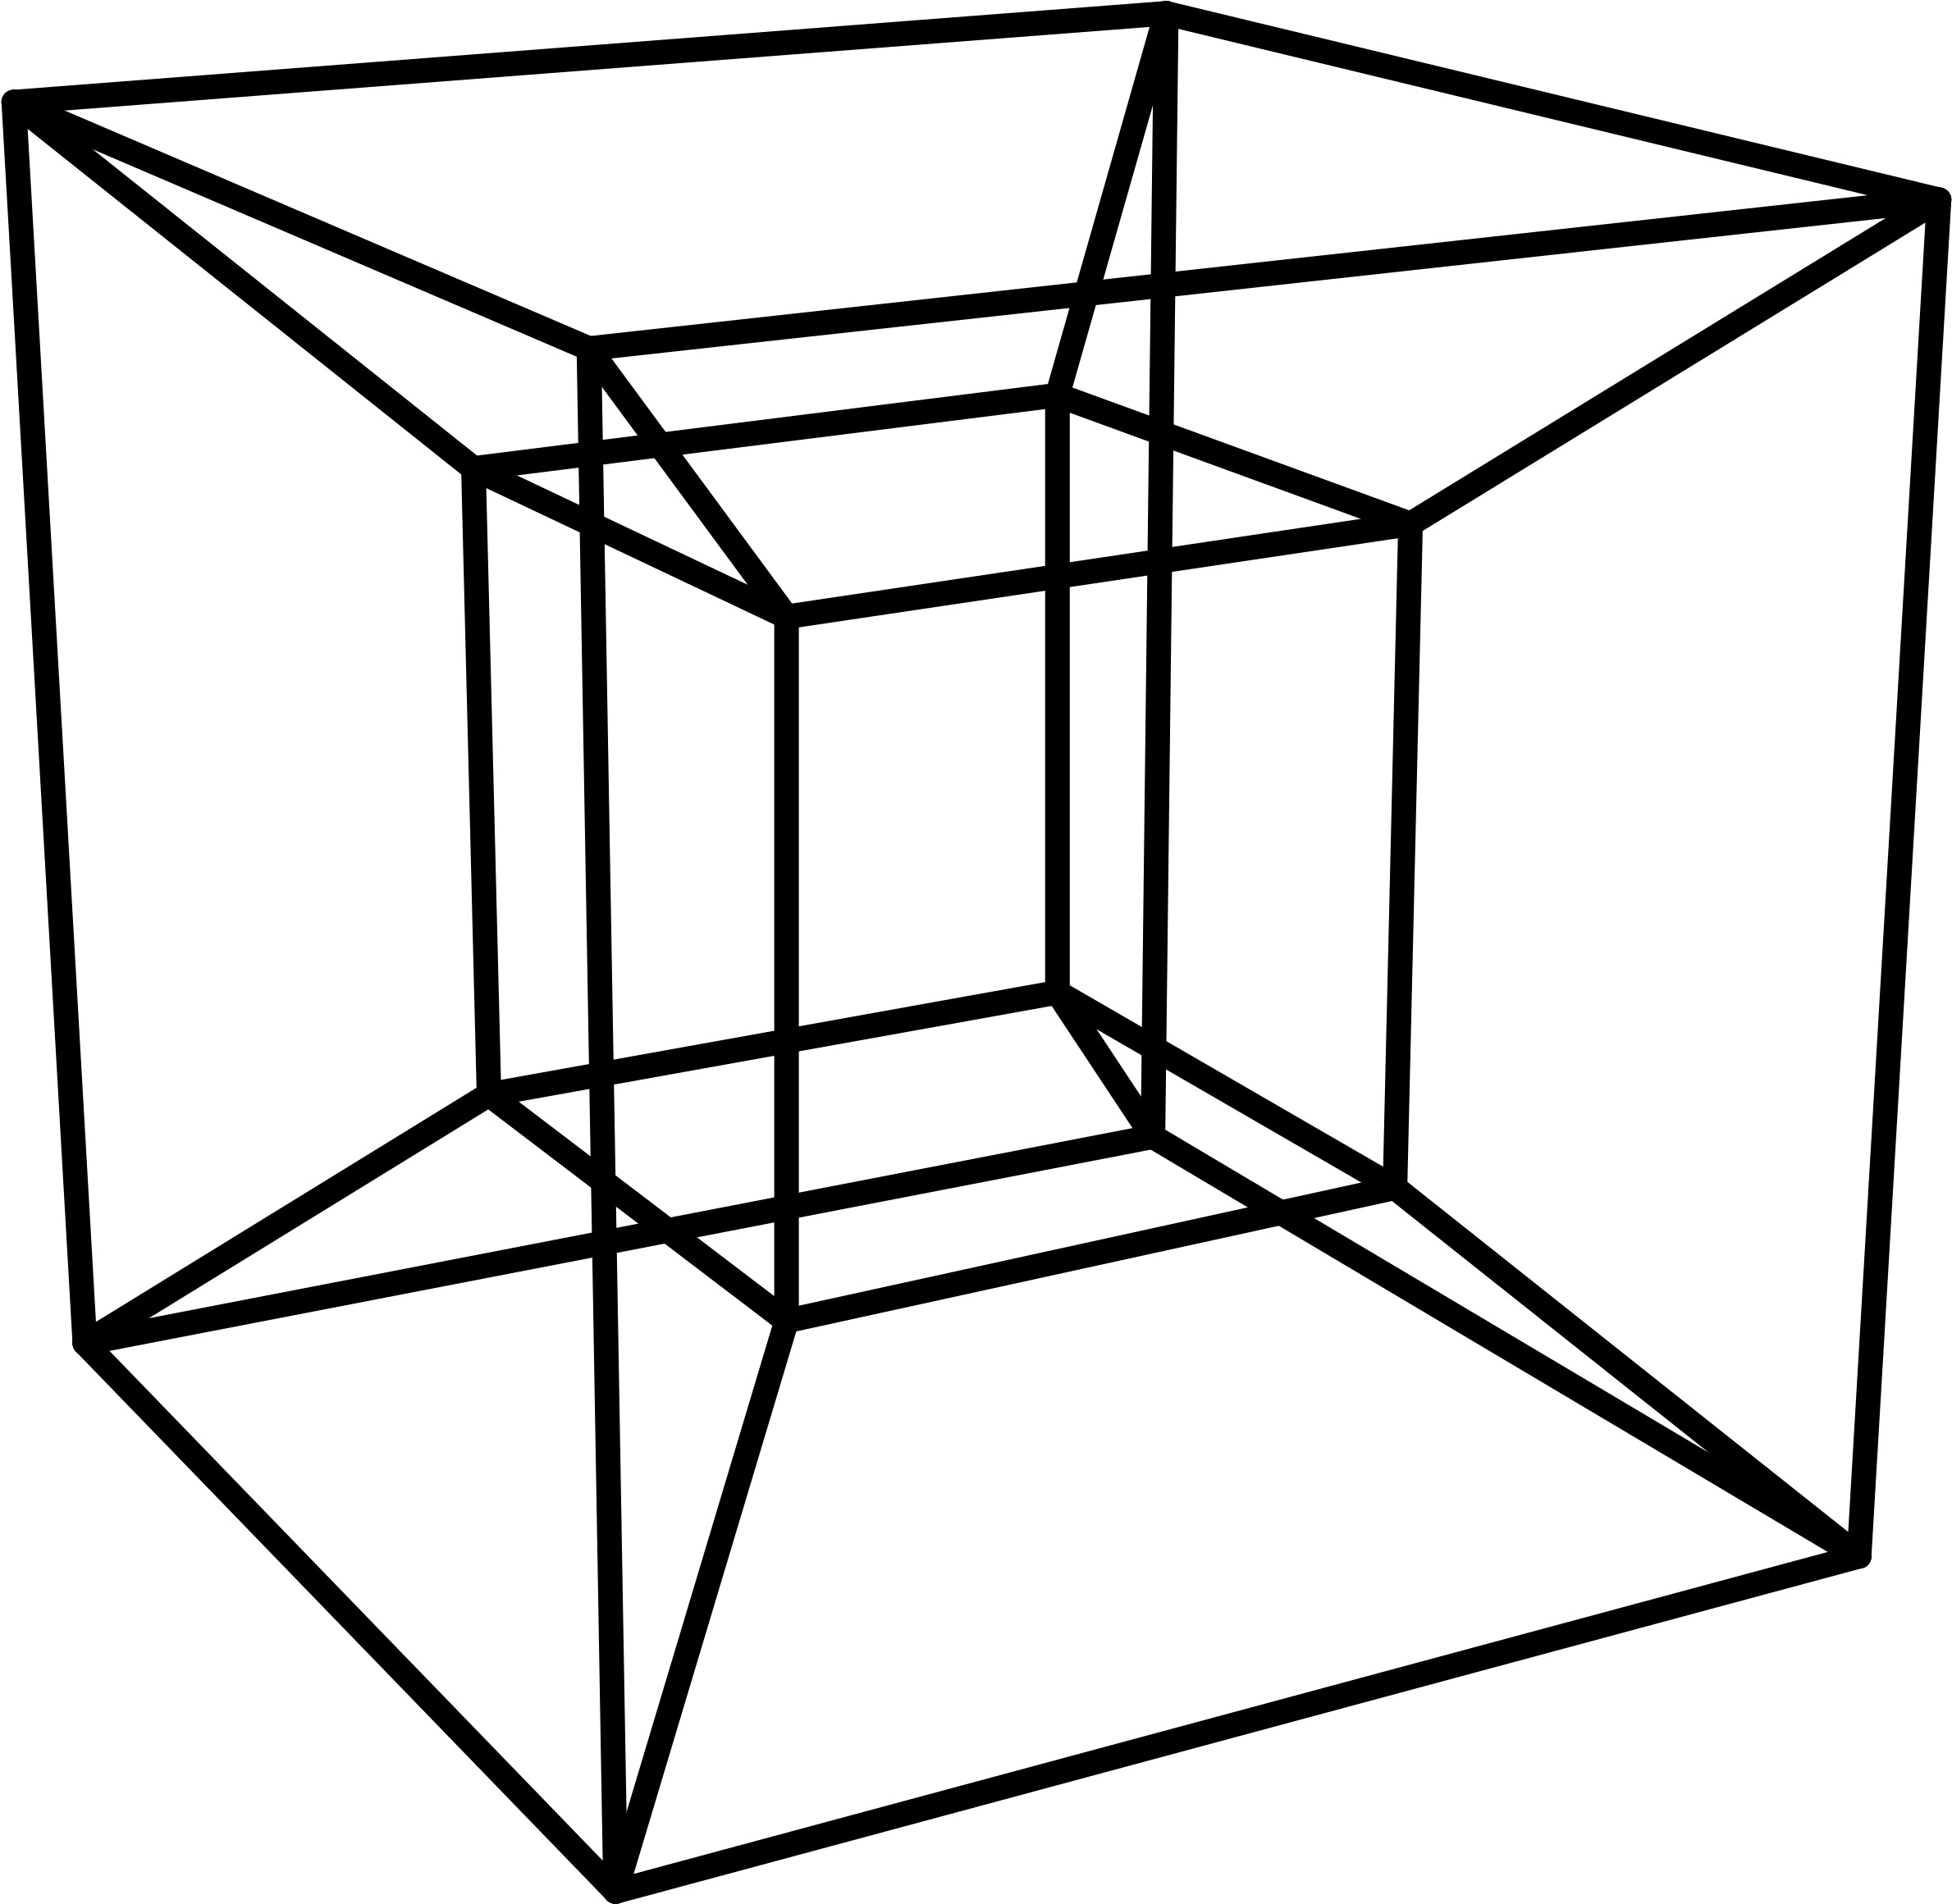
\includegraphics[width=10cm]{resources/1.png}\\[2.0cm]
    \end{figure}

    \begin{multicols}{2}
        \begin{flushright} \large

            {Выполнили студенты группы: 5130904/00104:}\\
            {\phantom{qwe}}\\
            {\phantom{qwe}}\\
            {\phantom{qwe}}\\
            {\phantom{qwe}}\\

            {Преподаватель:\\}

        \end{flushright}
        \begin{flushright}

            {Почернин В. С.}\\
            {Шиляев В. С.}\\
            {Мурзаканов И. М.}\\
            {Разукрантов В. Е.}\\[0.5cm]


            Маслаков А. П.\\

        \end{flushright}
    \end{multicols}

    \flushright{
        {\phantom{qwe}}\\[0.5cm]
    }
    \centering{
        Санкт-Петербург\\
        2023
    }

    \vfill
\end{titlepage}

\Large
\tableofcontents
\newpage
\large

\section{Макет дизайна интерфейса}

\begin{figure}[H]
    \centering
    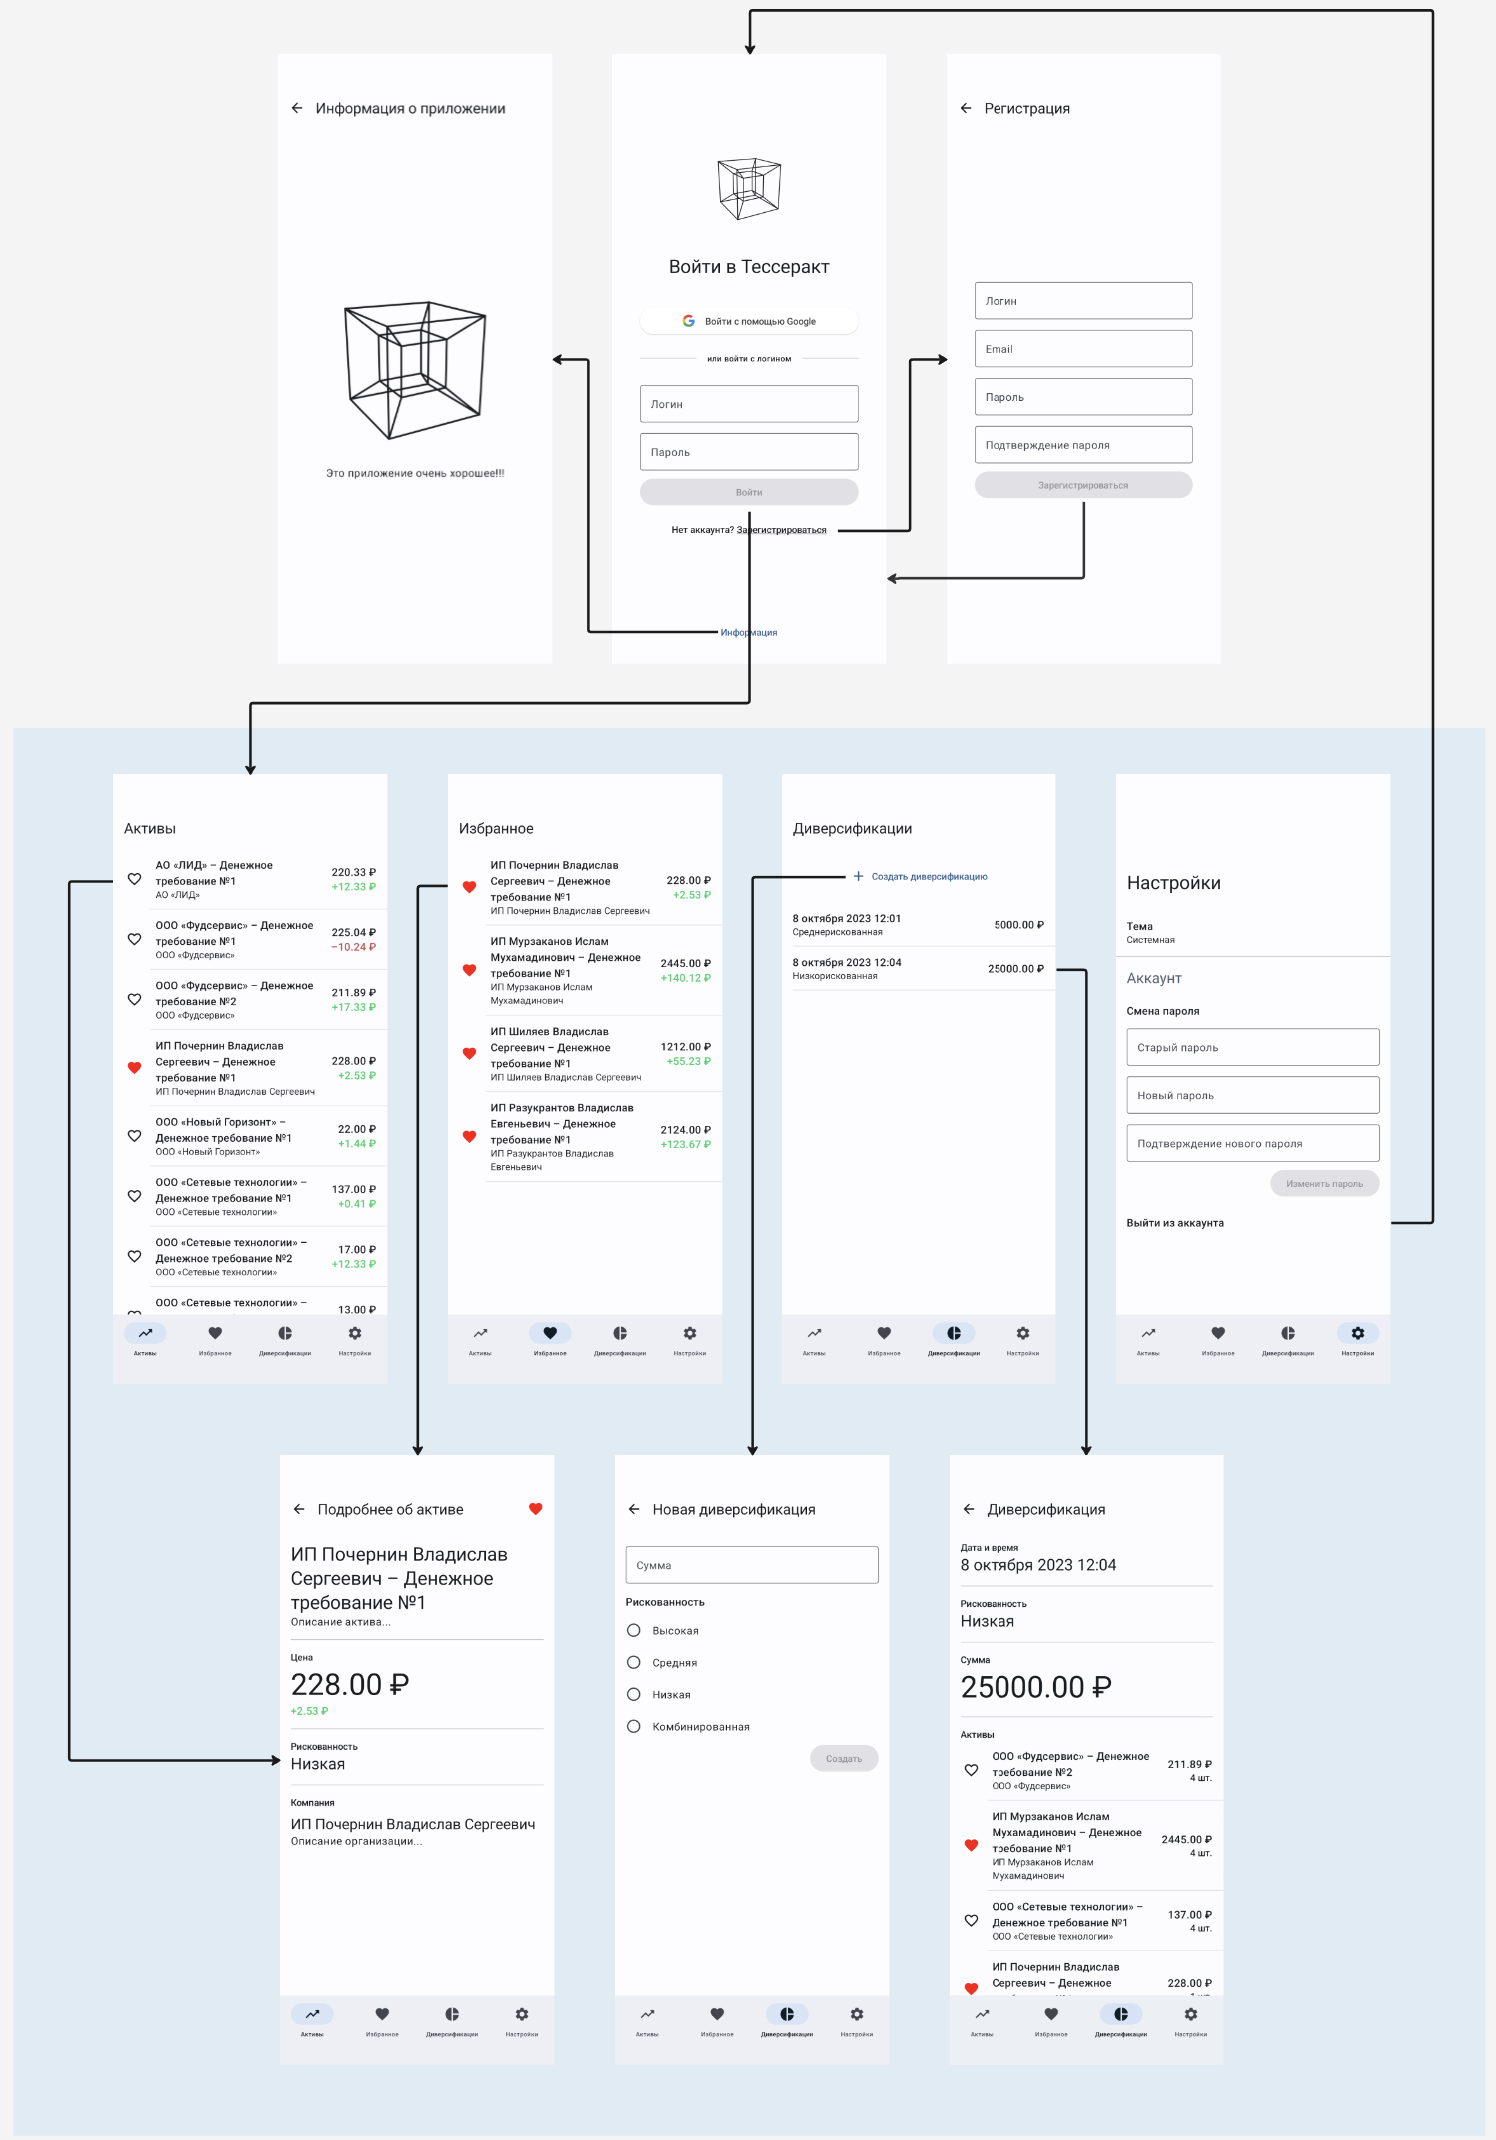
\includegraphics[width=17cm]{resources/3.png}
    \caption{Схема переходов между страницами}
\end{figure}

\subsection{Список страниц}

\begin{enumerate}
    \item Страница входа (LoginPage).
    \item Страница информации (InfoPage).
    \item Страница регистрации (RegistrationPage).
    \item Страница активов (AssetsPage).
    \item Страница конкретного актива (AssetPage).
    \item Страница избранных активов (FavouritesPage).
    \item Страница портфелей (PortfoliosPage).
    \item Страница создания портфеля (PortfolioCreatePage).
    \item Страница конкретного портфеля (PortfolioPage).
    \item Страница настроек (SettingsPage).
\end{enumerate}

\section{Архитектура приложения}

Клиентская часть приложения реализует паттерны \texttt{Single Activity Application}, а также \texttt{MVVM (Model View ViewModel)}.

Пользователь взаимодействует с UI, написанном на \texttt{Compose}, который в свою очередь получает данные из \texttt{ViewModel} и отправляет действия пользователя во \texttt{ViewModel}.

Клиент же общается с сервером посредством предоставляемого сервером API, внутри которого происходит исполнение бизнес-логики и обращение к БД.

Используется модель MVC.

\begin{figure}[H]
    \centering
    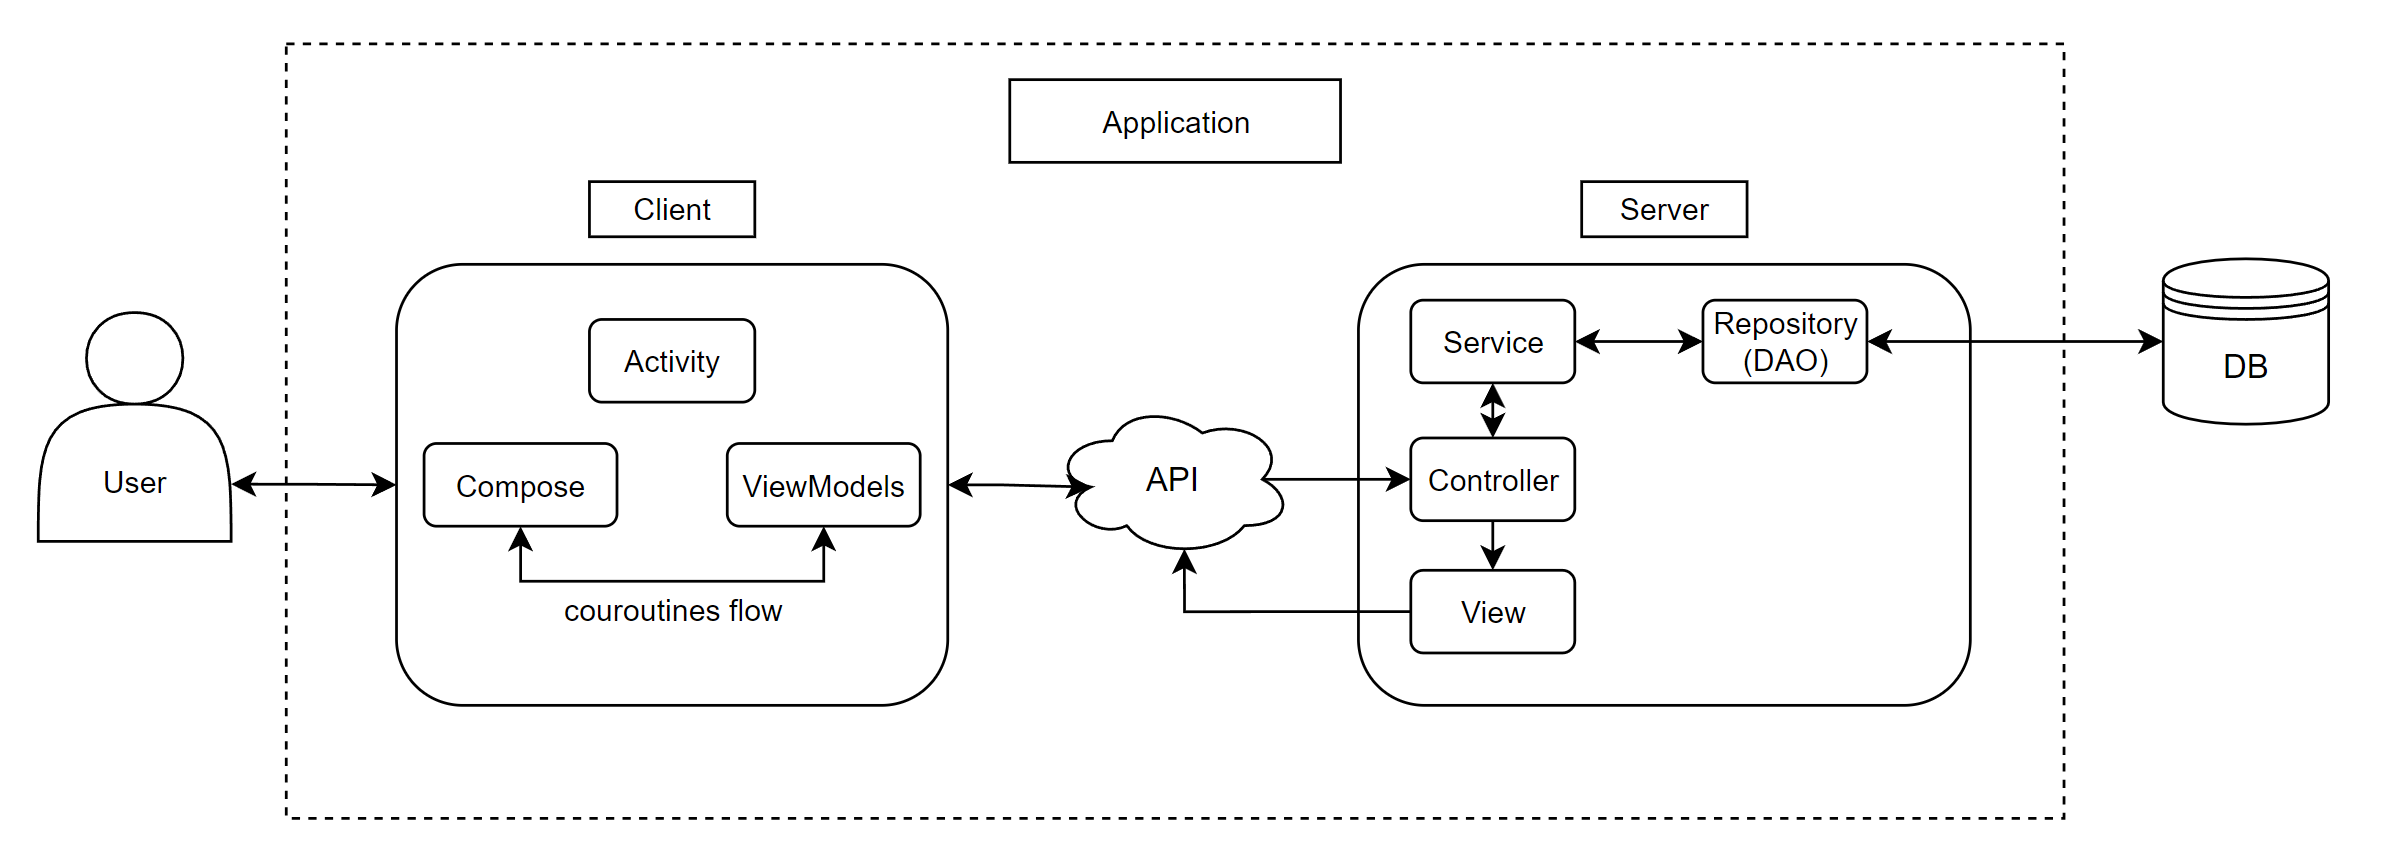
\includegraphics[width=19cm]{resources/2.png}
    \caption{Архитектура приложения}
\end{figure}

\section{Стек технологий}

\subsection{Backend}

\begin{itemize}
    \item \textbf{Java} - язык программирования.
    \item \textbf{Spring Boot} - основной фреймворк.
    \item \textbf{Spring Web MVC} - веб среда Spring для работы с сетью.
    \item \textbf{Spring Security} - фреймворк, предоставляющий механизмы построения систем аутентификации и авторизации.
    \item \textbf{Spring Data JPA} - механизм для взаимодействия с сущностями базы данных.
    \item \textbf{PostgreSQL} - система управления базами данных.
    \item \textbf{Flyway} - система управления версиями баз данных.
    \item \textbf{Swagger} - инструмент для описания API.
\end{itemize}

\subsection{Frontend}

\begin{itemize}
    \item \textbf{Kotlin} - язык программирования.
    \item \textbf{Kotlin Coroutines} - библиотека для асинхронной работы.
    \item \textbf{Ktor} - библиотека для работы с API.
    \item \textbf{Koin} - DI (Dependency Injection) фреймворк.
    \item \textbf{Compose} - библиотека для UI.
\end{itemize}

\section{Диаграмма классов}

\begin{figure}[H]
    \centering
    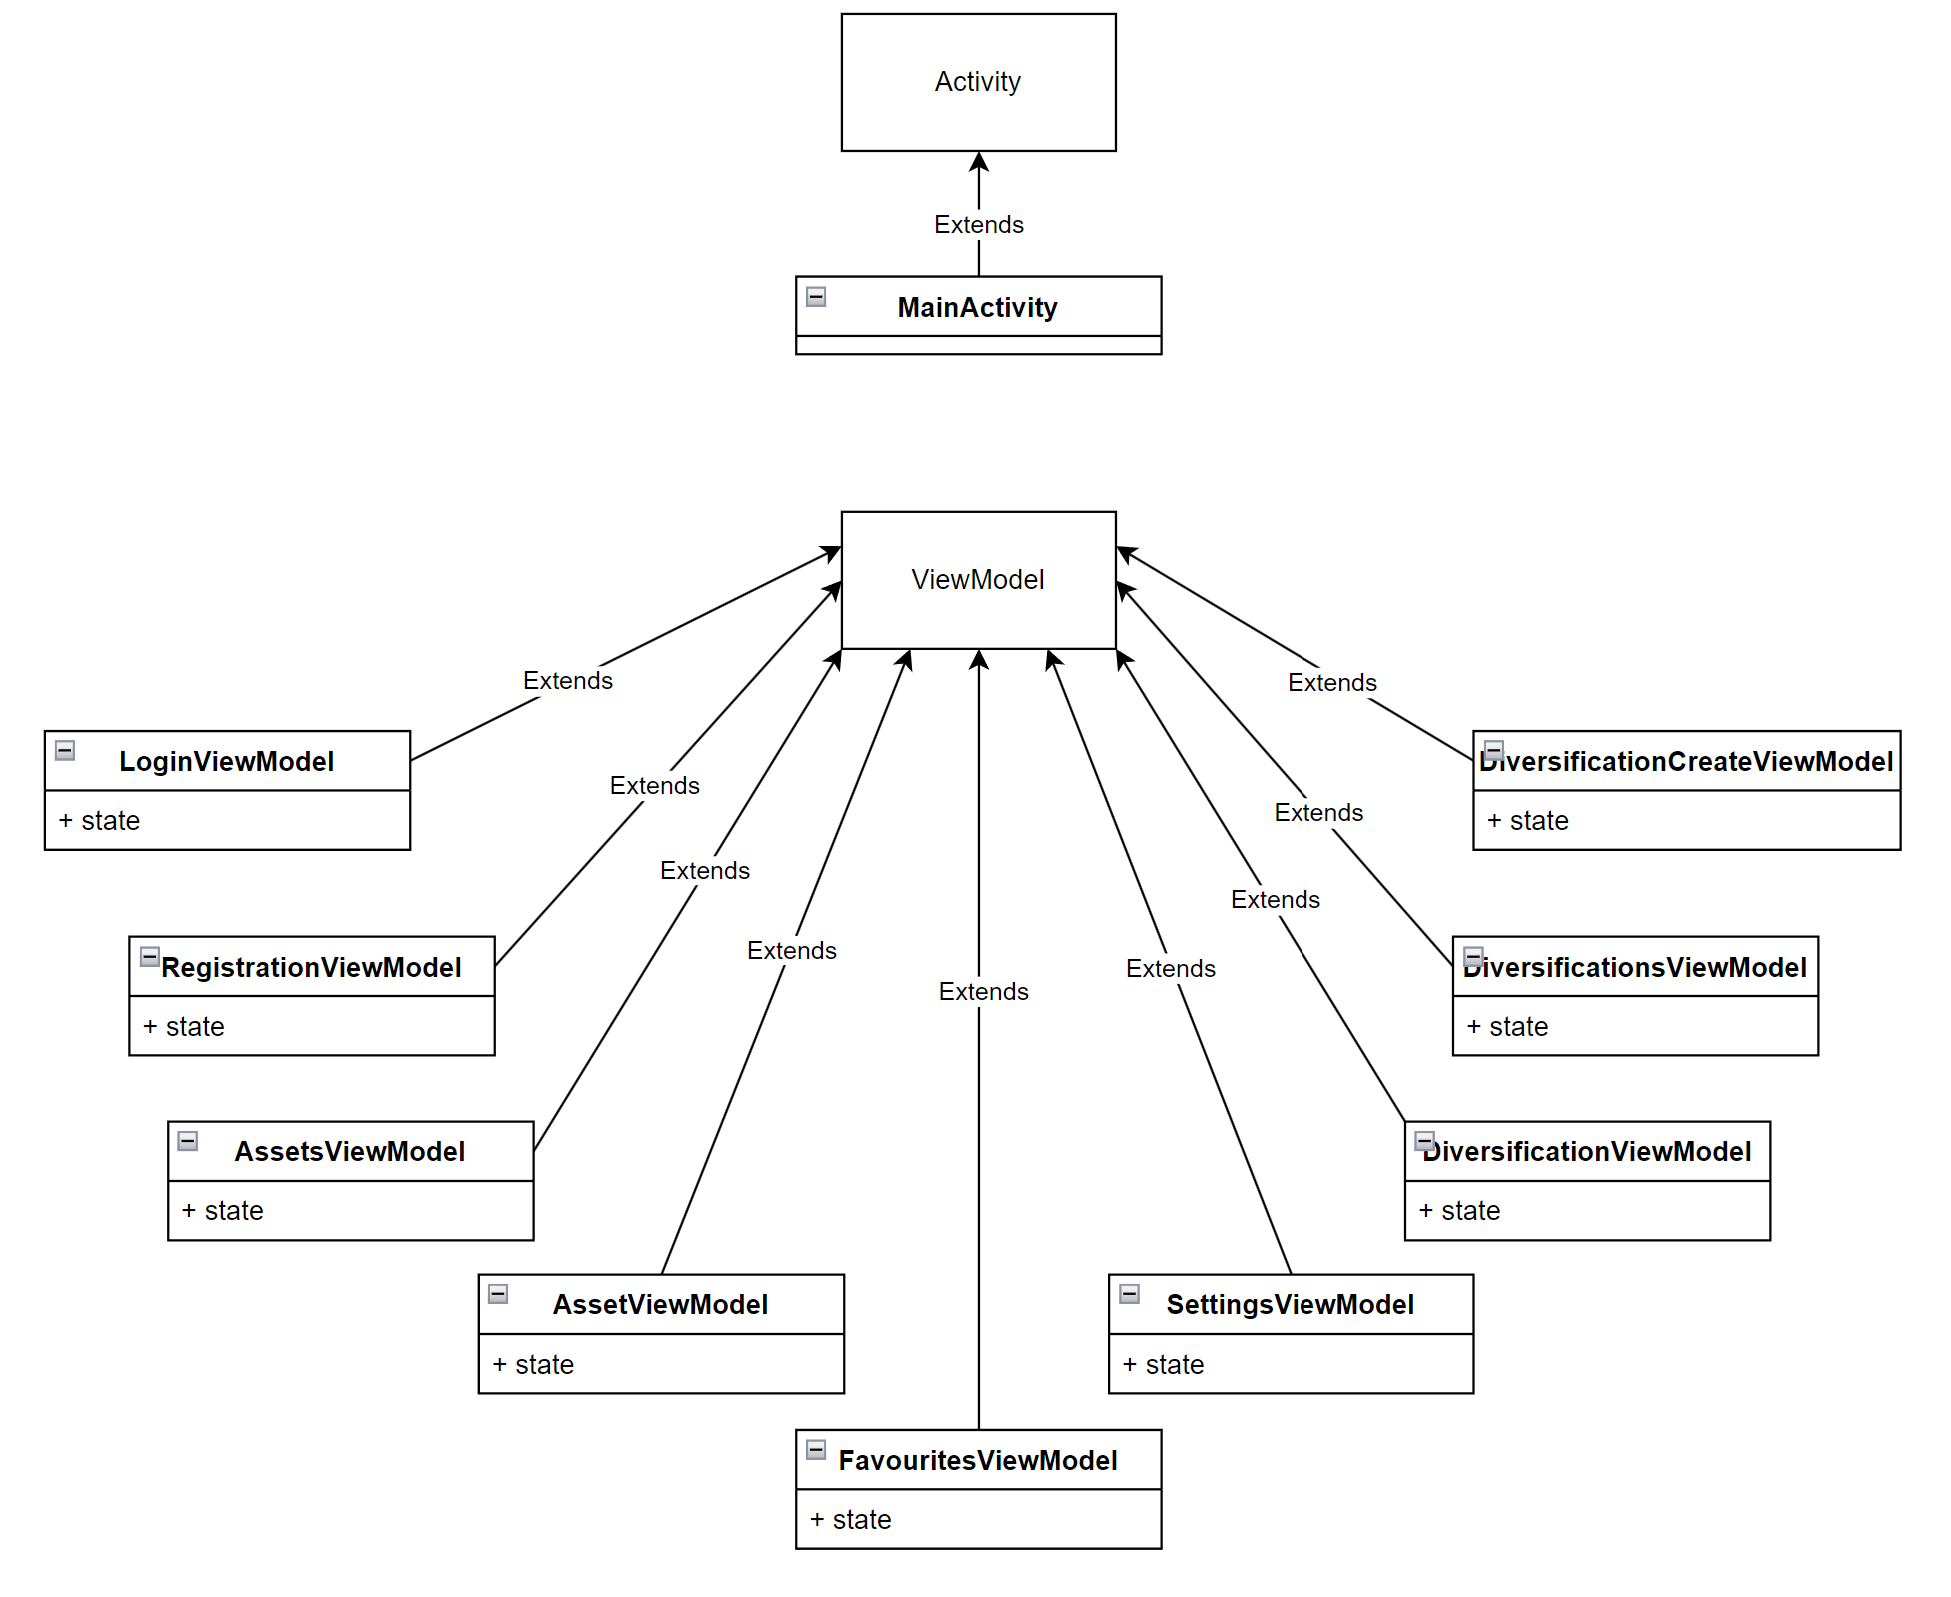
\includegraphics[width=17cm]{resources/15.png}
    \caption{Диаграмма классов клиентского приложения}
\end{figure}

\begin{figure}[H]
    \centering
    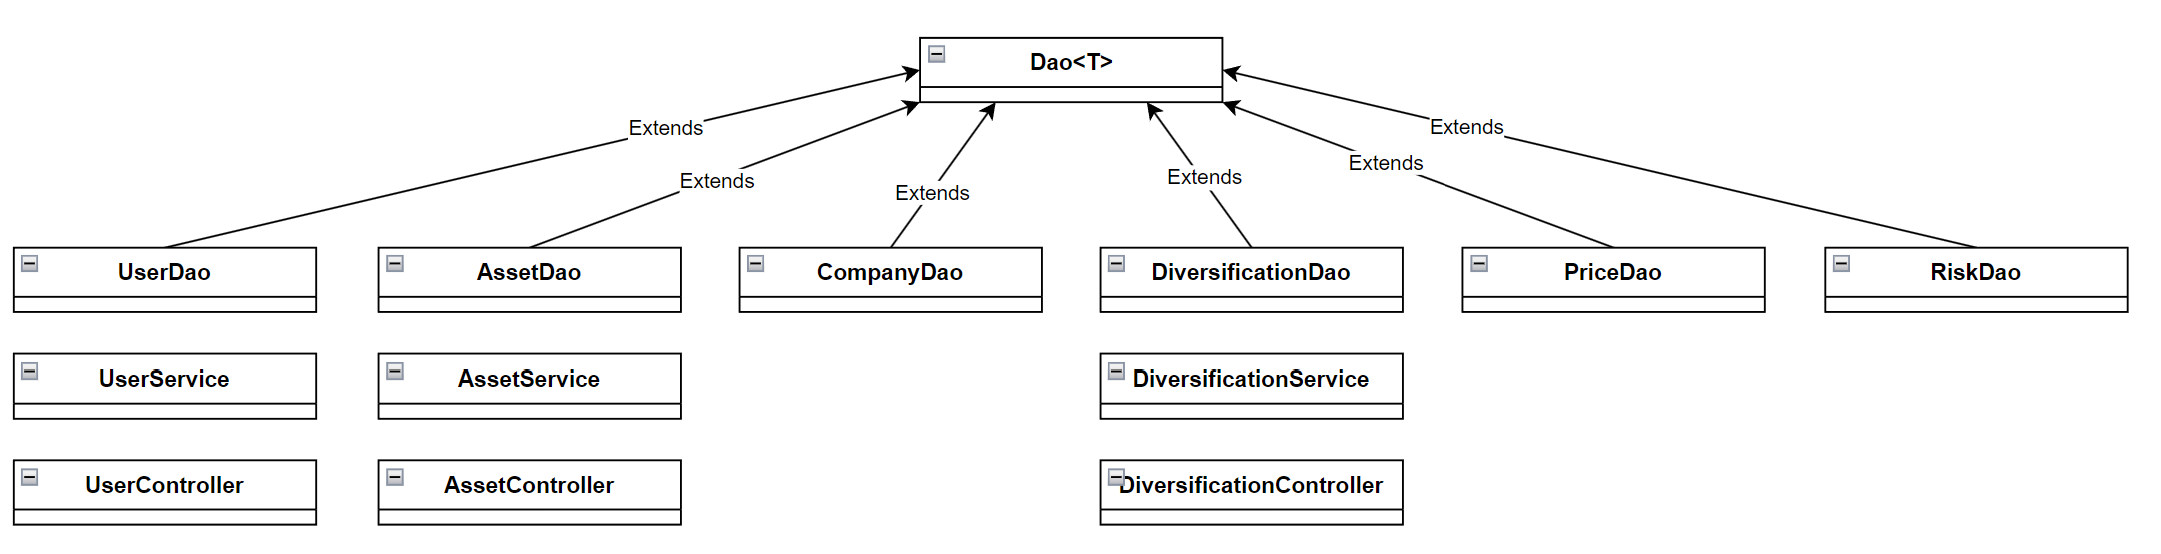
\includegraphics[width=17cm]{resources/16.png}
    \caption{Диаграмма классов серверного приложения}
\end{figure}

\section{Схема базы данных}


\begin{figure}[H]
    \centering
    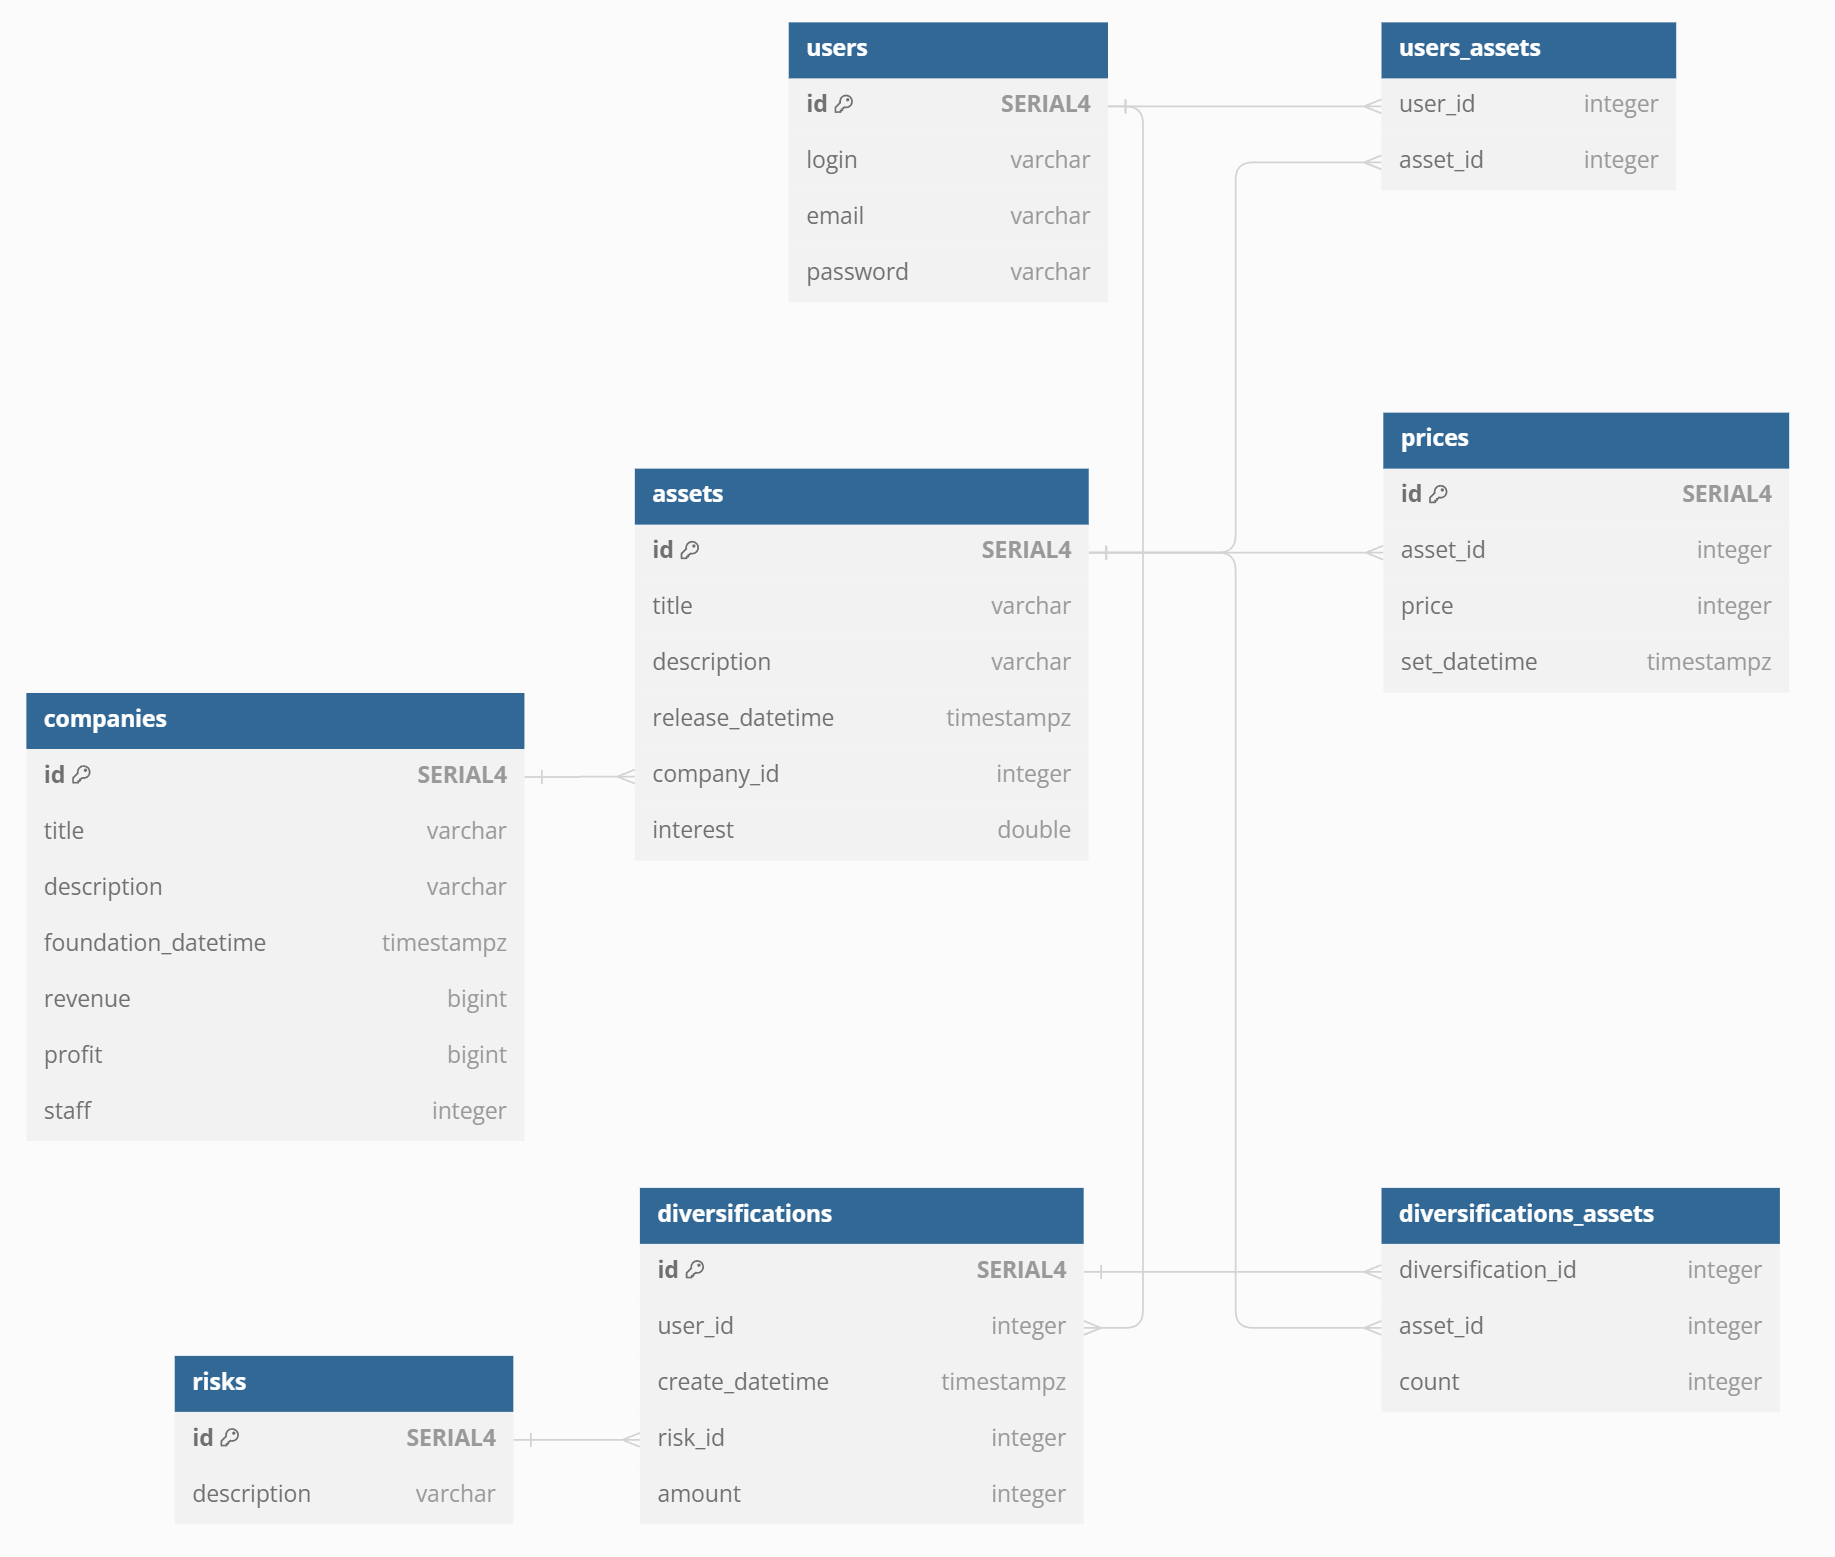
\includegraphics[width=17cm]{resources/14.png}
    \caption{Схема базы данных}
\end{figure}

\section{API}

API будет поддерживать следующие HTTP коды:
\begin{itemize}
    \item \texttt{200 OK} - успешные \texttt{GET}, \texttt{PUT}, \texttt{DELETE} или \texttt{POST} без создания.
    \item \texttt{201 Created} - успешный \texttt{POST} с созданием.
    \item \texttt{400 Bad Request} - некорректное тело запроса.
    \item \texttt{401 Unauthorized} - отсутствуют данные аутентификации.
    \item \texttt{404 Not Found} - запрашивается несуществующий ресурс.
    \item \texttt{500 Internal Server Error} - непредвиденная ошибка.
\end{itemize}

\subsection{Аутентификация через логин и пароль}

\begin{itemize}
    \item HTTP метод: \texttt{GET}.
    \item Путь: \texttt{/login/tesseract}.
    \item Входные параметры:
    \begin{itemize}
        \item Тело (JSON):
        \begin{itemize}
            \item String login;
            \item String password;
        \end{itemize}
    \end{itemize}
    \item Выходные параметры:
    \begin{itemize}
        \item Тело (JSON):
        \begin{itemize}
            \item String token;
        \end{itemize}
        \item HTTP коды:
        \begin{itemize}
            \item \texttt{200 OK} - успешная авторизация.
            \item \texttt{400 Bad Request} - некорректное тело запроса.
            \item \texttt{401 Unauthorized} - несуществующая комбинация логин/пароль.
            \item \texttt{500 Internal Server Error} - непредвиденная ошибка.
        \end{itemize}
    \end{itemize}
\end{itemize}

\subsection{Аутентификация через Google OAuth}

\begin{itemize}
    \item HTTP метод: \texttt{GET}.
    \item Путь: \texttt{/login/google}.
    \item Входные параметры:
    \begin{itemize}
        \item Тело (JSON):
        \begin{itemize}
            \item String googleToken;
        \end{itemize}
    \end{itemize}
    \item Выходные параметры:
    \begin{itemize}
        \item Тело (JSON):
        \begin{itemize}
            \item String token;
        \end{itemize}
        \item HTTP коды:
        \begin{itemize}
            \item \texttt{200 OK} - успешная авторизация.
            \item \texttt{400 Bad Request} - некорректное тело запроса.
            \item \texttt{401 Unauthorized} - некорректный Google токен.
            \item \texttt{500 Internal Server Error} - непредвиденная ошибка.
        \end{itemize}
    \end{itemize}
\end{itemize}

\subsection{Регистрация пользователя}

\begin{itemize}
    \item HTTP метод: \texttt{POST}.
    \item Путь: \texttt{/users}.
    \item Входные параметры:
    \begin{itemize}
        \item Тело (JSON):
        \begin{itemize}
            \item String login;
            \item String password;
            \item String email;
        \end{itemize}
    \end{itemize}
    \item Выходные параметры:
    \begin{itemize}
        \item HTTP коды:
        \begin{itemize}
            \item \texttt{201 Created} - успешная регистрация.
            \item \texttt{400 Bad Request} - некорректное тело запроса.
            \item \texttt{500 Internal Server Error} - непредвиденная ошибка.
        \end{itemize}
    \end{itemize}
\end{itemize}

\subsection{Получить список всех активов}

\begin{itemize}
    \item HTTP метод: \texttt{GET}.
    \item Путь: \texttt{/assets}.
    \item Входные параметры:
    \begin{itemize}
        \item Заголовок: данные аутентификации;
        \item Строка запроса: id последнего загруженного актива (опционально).
    \end{itemize}
    \item Выходные параметры:
    \begin{itemize}
        \item Тело (JSON) - список:
        \begin{itemize}
            \item String assetTitle; - название актива.
            \item String companyTitle; - название компании.
            \item Integer assetPrice; - стоимость актива.
            \item Integer assetDiff; - изменение стоимости актива за последний месяц.
            \item Boolean favouriteStatus; - статус избранного актива.
        \end{itemize}
        \item HTTP коды:
        \begin{itemize}
            \item \texttt{200 OK} - успешное получение списка активов.
            \item \texttt{400 Bad Request} - некорректное тело запроса.
            \item \texttt{401 Unauthorized} - отсутствуют данные аутентификации.
            \item \texttt{500 Internal Server Error} - непредвиденная ошибка.
        \end{itemize}
    \end{itemize}
\end{itemize}

\subsection{Добавить актив в избранное}

\begin{itemize}
    \item HTTP метод: \texttt{POST}.
    \item Путь: \texttt{favourites/\{id\}}.
    \item Входные параметры:
    \begin{itemize}
        \item Заголовок: данные аутентификации.
        \item Путь: id добавляемого в избранное актива.
    \end{itemize}
    \item Выходные параметры:
    \begin{itemize}
        \item HTTP коды:
        \begin{itemize}
            \item \texttt{200 OK} - успешное добавление актива в избранное, если он там уже был.
            \item \texttt{201 Created} - успешное добавление актива в избранное.
            \item \texttt{400 Bad Request} - некорректное тело запроса.
            \item \texttt{401 Unauthorized} - отсутствуют данные аутентификации.
            \item \texttt{404 Not Found} - указан несуществующий id актива.
            \item \texttt{500 Internal Server Error} - непредвиденная ошибка.
        \end{itemize}
    \end{itemize}
\end{itemize}

\subsection{Удалить актив из избранного}

\begin{itemize}
    \item HTTP метод: \texttt{DELETE}.
    \item Путь: \texttt{favourites/\{id\}}.
    \item Входные параметры:
    \begin{itemize}
        \item Заголовок: данные аутентификации.
        \item Путь: id удаляемого из избранного актива.
    \end{itemize}
    \item Выходные параметры:
    \begin{itemize}
        \item HTTP коды:
        \begin{itemize}
            \item \texttt{200 OK} - успешное удаление актива из избранного (либо отсутствие соответствующего id актива).
            \item \texttt{400 Bad Request} - некорректное тело запроса.
            \item \texttt{401 Unauthorized} - отсутствуют данные аутентификации.
            \item \texttt{500 Internal Server Error} - непредвиденная ошибка.
        \end{itemize}
    \end{itemize}
\end{itemize}

\subsection{Получить информацию о конкретном активе}

\begin{itemize}
    \item HTTP метод: \texttt{GET}.
    \item Путь: \texttt{/assets/\{id\}}.
    \item Входные параметры:
    \begin{itemize}
        \item Заголовок: данные аутентификации.
        \item Путь: id запрашиваемого актива.
    \end{itemize}
    \item Выходные параметры:
    \begin{itemize}
        \item Тело (JSON):
        \begin{itemize}
            \item String assetTitle; - название актива.
            \item String assetDescription; - описание актива.
            \item Integer assetPrice; - стоимость актива.
            \item Integer assetDiff; - изменение стоимости актива за последний месяц.
            \item String companyTitle; - название компании.
            \item String companyDescription; - описание компании.
            \item Integer risk; - степень рискованности актива.
            \item Boolean favouriteStatus; - статус избранного актива.
        \end{itemize}
        \item HTTP коды:
        \begin{itemize}
            \item \texttt{200 OK} - успешное получение информации об активе.
            \item \texttt{400 Bad Request} - некорректное тело запроса.
            \item \texttt{401 Unauthorized} - отсутствуют данные аутентификации.
            \item \texttt{404 Not Found} - отсутствие запрашиваемого id актива.
            \item \texttt{500 Internal Server Error} - непредвиденная ошибка.
        \end{itemize}
    \end{itemize}
\end{itemize}

\subsection{Получить список избранных активов}

\begin{itemize}
    \item HTTP метод: \texttt{GET}.
    \item Путь: \texttt{/favourites}.
    \item Входные параметры:
    \begin{itemize}
        \item Заголовок: данные аутентификации.
        \item Строка запроса: id последнего загруженного избранного актива (опционально).
    \end{itemize}
    \item Выходные параметры:
    \begin{itemize}
        \item Тело (JSON) - список:
        \begin{itemize}
            \item String assetTitle; - название актива.
            \item String companyTitle; - название компании.
            \item Integer assetPrice; - стоимость актива.
            \item Integer assetDiff; - изменение стоимости актива за последний месяц.
            \item Boolean favouriteStatus; - статус избранного актива.
        \end{itemize}
        \item HTTP коды:
        \begin{itemize}
            \item \texttt{200 OK} - успешное получение списка активов.
            \item \texttt{400 Bad Request} - некорректное тело запроса.
            \item \texttt{401 Unauthorized} - отсутствуют данные аутентификации.
            \item \texttt{500 Internal Server Error} - непредвиденная ошибка.
        \end{itemize}
    \end{itemize}
\end{itemize}

\subsection{Получить список портфелей}

\begin{itemize}
    \item HTTP метод: \texttt{GET}.
    \item Путь: \texttt{/portfolios}.
    \item Входные параметры:
    \begin{itemize}
        \item Заголовок: данные аутентификации.
        \item Строка запроса: id последнего загруженного портфеля (опционально).
    \end{itemize}
    \item Выходные параметры:
    \begin{itemize}
        \item Тело (JSON) - список:
        \begin{itemize}
            \item Timestamp createDatetime; - дата и время создания портфеля.
            \item Integer risk; - степень рискованности портфеля.
            \item Integer amount; - стоимость портфеля.
        \end{itemize}
        \item HTTP коды:
        \begin{itemize}
            \item \texttt{200 OK} - успешное получение списка портфелей.
            \item \texttt{400 Bad Request} - некорректное тело запроса.
            \item \texttt{401 Unauthorized} - отсутствуют данные аутентификации.
            \item \texttt{500 Internal Server Error} - непредвиденная ошибка.
        \end{itemize}
    \end{itemize}
\end{itemize}

\subsection{Создать портфель}

\begin{itemize}
    \item HTTP метод: \texttt{POST}.
    \item Путь: \texttt{/portfolios}.
    \item Входные параметры:
    \begin{itemize}
        \item Заголовок: данные аутентификации.
        \item Тело (JSON):
        \begin{itemize}
            \item Integer amount; - стоимость создаваемого портфеля.
            \item Integer risk; - степень рискованности создаваемого портфеля.
        \end{itemize}
    \end{itemize}
    \item Выходные параметры:
    \begin{itemize}
        \item HTTP коды:
        \begin{itemize}
            \item \texttt{201 Created} - успешное создание портфеля.
            \item \texttt{400 Bad Request} - некорректное тело запроса.
            \item \texttt{401 Unauthorized} - отсутствуют данные аутентификации.
            \item \texttt{500 Internal Server Error} - непредвиденная ошибка.
        \end{itemize}
    \end{itemize}
\end{itemize}

\subsection{Получить информацию о конкретном портфеле}

\begin{itemize}
    \item HTTP метод: \texttt{GET}.
    \item Путь: \texttt{/portfolios/\{id\}}.
    \item Входные параметры:
    \begin{itemize}
        \item Заголовок: данные аутентификации.
        \item Путь: id запрашиваемого портфеля.
    \end{itemize}
    \item Выходные параметры:
    \begin{itemize}
        \item Тело (JSON):
        \begin{itemize}
            \item Timestamp createDatetime; - дата и время создания портфеля.
            \item Integer risk; - уровень рискованности портфеля.
            \item Integer amount - стоимость портфеля.
            \item Список:
            \begin{itemize}
                \item String assetTitle; - название актива.
                \item String companyTitle; - название компании.
                \item Integer priceSum; - \textbf{старая} цена актива (то есть цена на момент создания портфеля).
                \item Integer count; количество активов данного вида.
            \end{itemize}
        \end{itemize}
        \item HTTP коды:
        \begin{itemize}
            \item \texttt{200 OK} - успешное получение портфеля.
            \item \texttt{400 Bad Request} - некорректное тело запроса.
            \item \texttt{401 Unauthorized} - отсутствуют данные аутентификации.
            \item \texttt{404 Not Found} - отсутствует портфель с таким id (либо запрашиваем не свой портфель).
            \item \texttt{500 Internal Server Error} - непредвиденная ошибка.
        \end{itemize}
    \end{itemize}
\end{itemize}

\subsection{Изменить пароль}

\begin{itemize}
    \item HTTP метод: \texttt{PUT}.
    \item Путь: \texttt{/users}.
    \item Входные параметры:
    \begin{itemize}
        \item Заголовок: данные аутентификации.
        \item Тело (JSON):
        \begin{itemize}
            \item String oldPassword; - старый пароль.
            \item String newPassword; - новый пароль.
        \end{itemize}
    \end{itemize}
    \item Выходные параметры:
    \begin{itemize}
        \item HTTP коды:
        \begin{itemize}
            \item \texttt{200 OK} - успешное изменение пароля.
            \item \texttt{400 Bad Request} - некорректное тело запроса.
            \item \texttt{401 Unauthorized} - отсутствуют данные аутентификации.
            \item \texttt{500 Internal Server Error} - внутренняя ошибка сервера.
        \end{itemize}
    \end{itemize}
\end{itemize}

\newpage
\section{Приложение 1: список страниц (экранов)}

\begin{figure}[H]
    \centering
    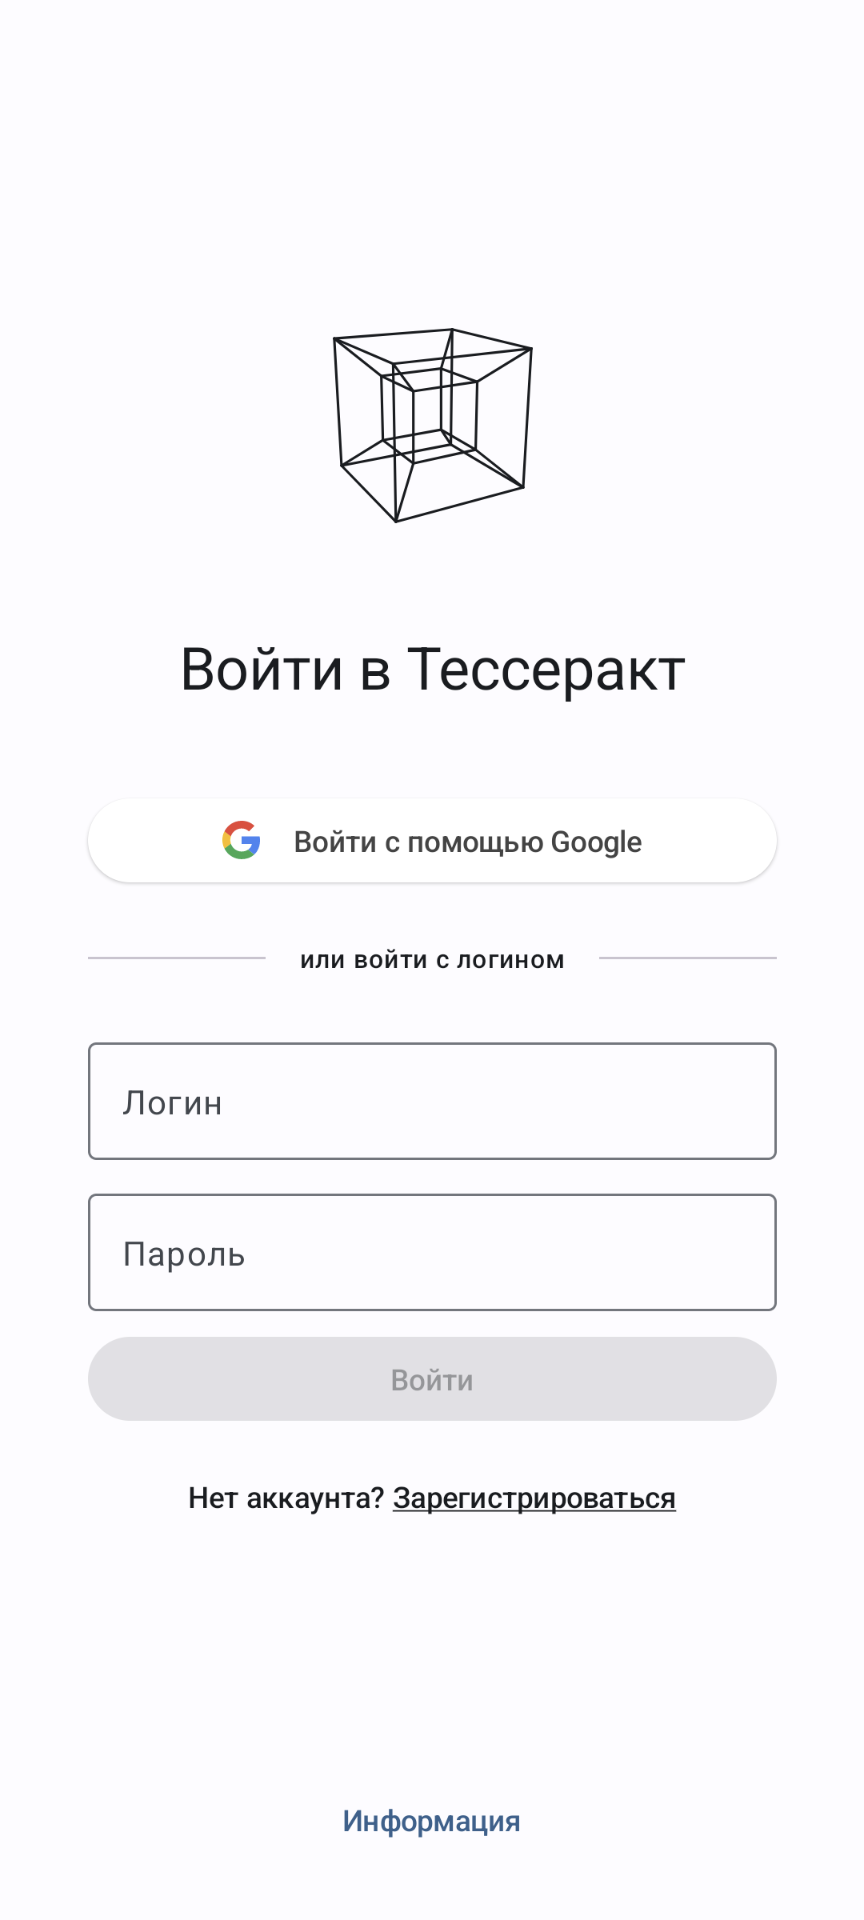
\includegraphics[width=5cm]{resources/4.png}
    \caption{Страница входа (LoginPage)}
\end{figure}

\begin{figure}[H]
    \centering
    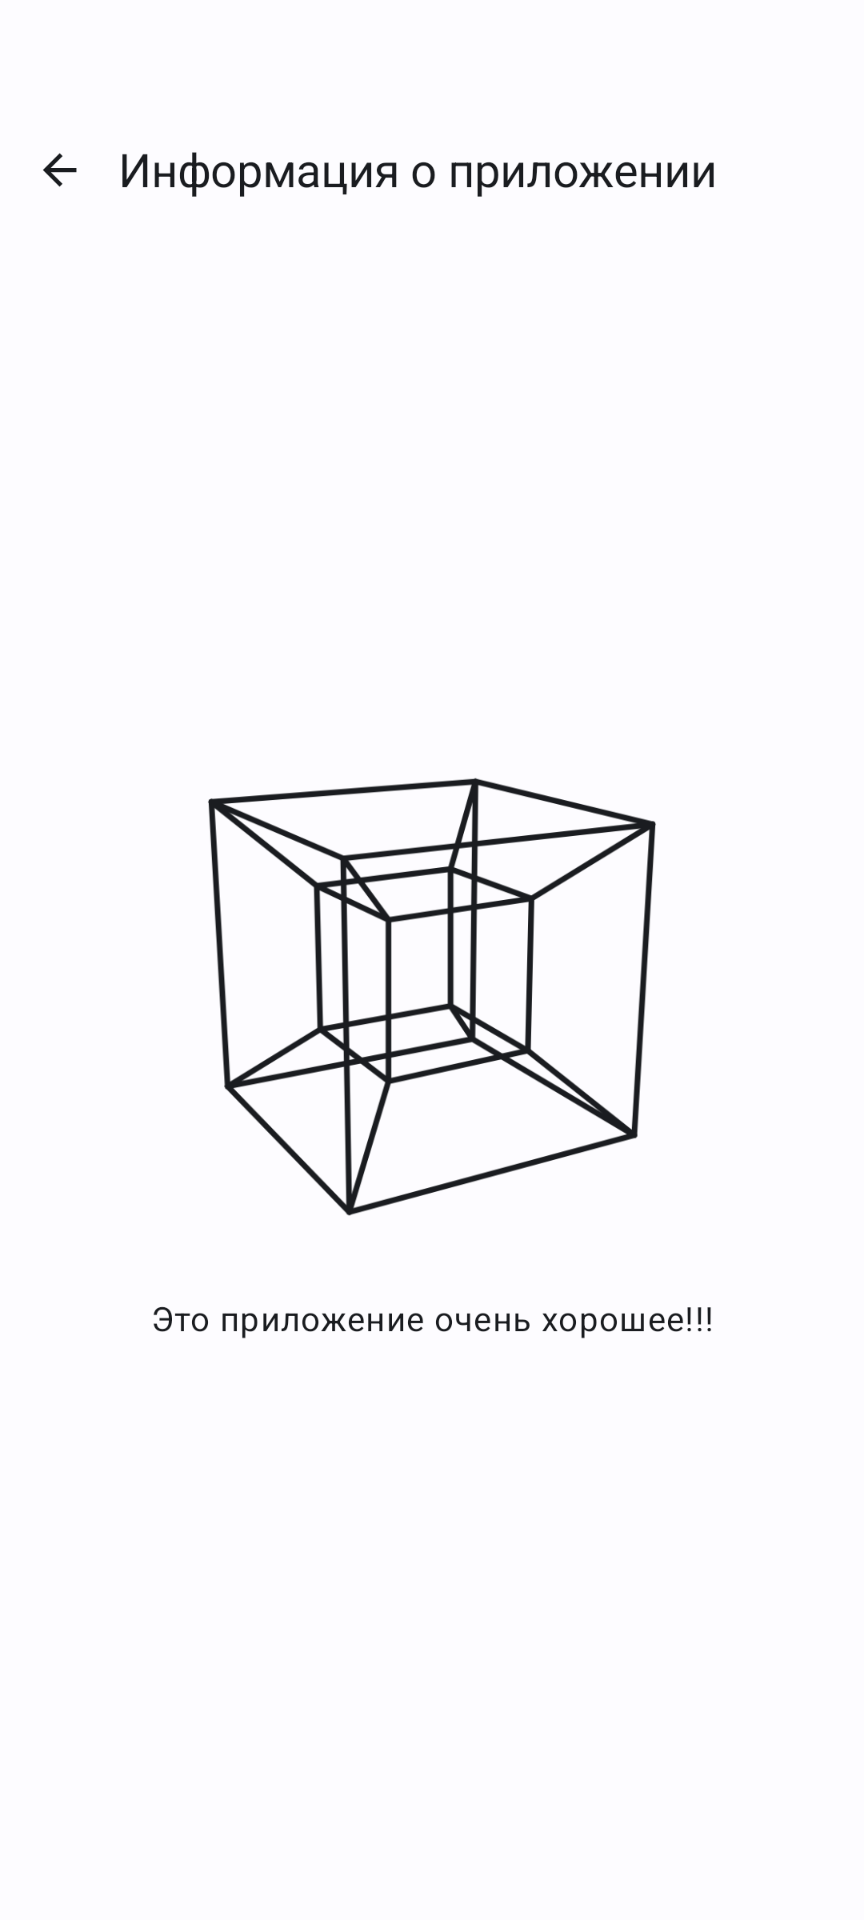
\includegraphics[width=5cm]{resources/5.png}
    \caption{Страница информации (InfoPage)}
\end{figure}

\begin{figure}[H]
    \centering
    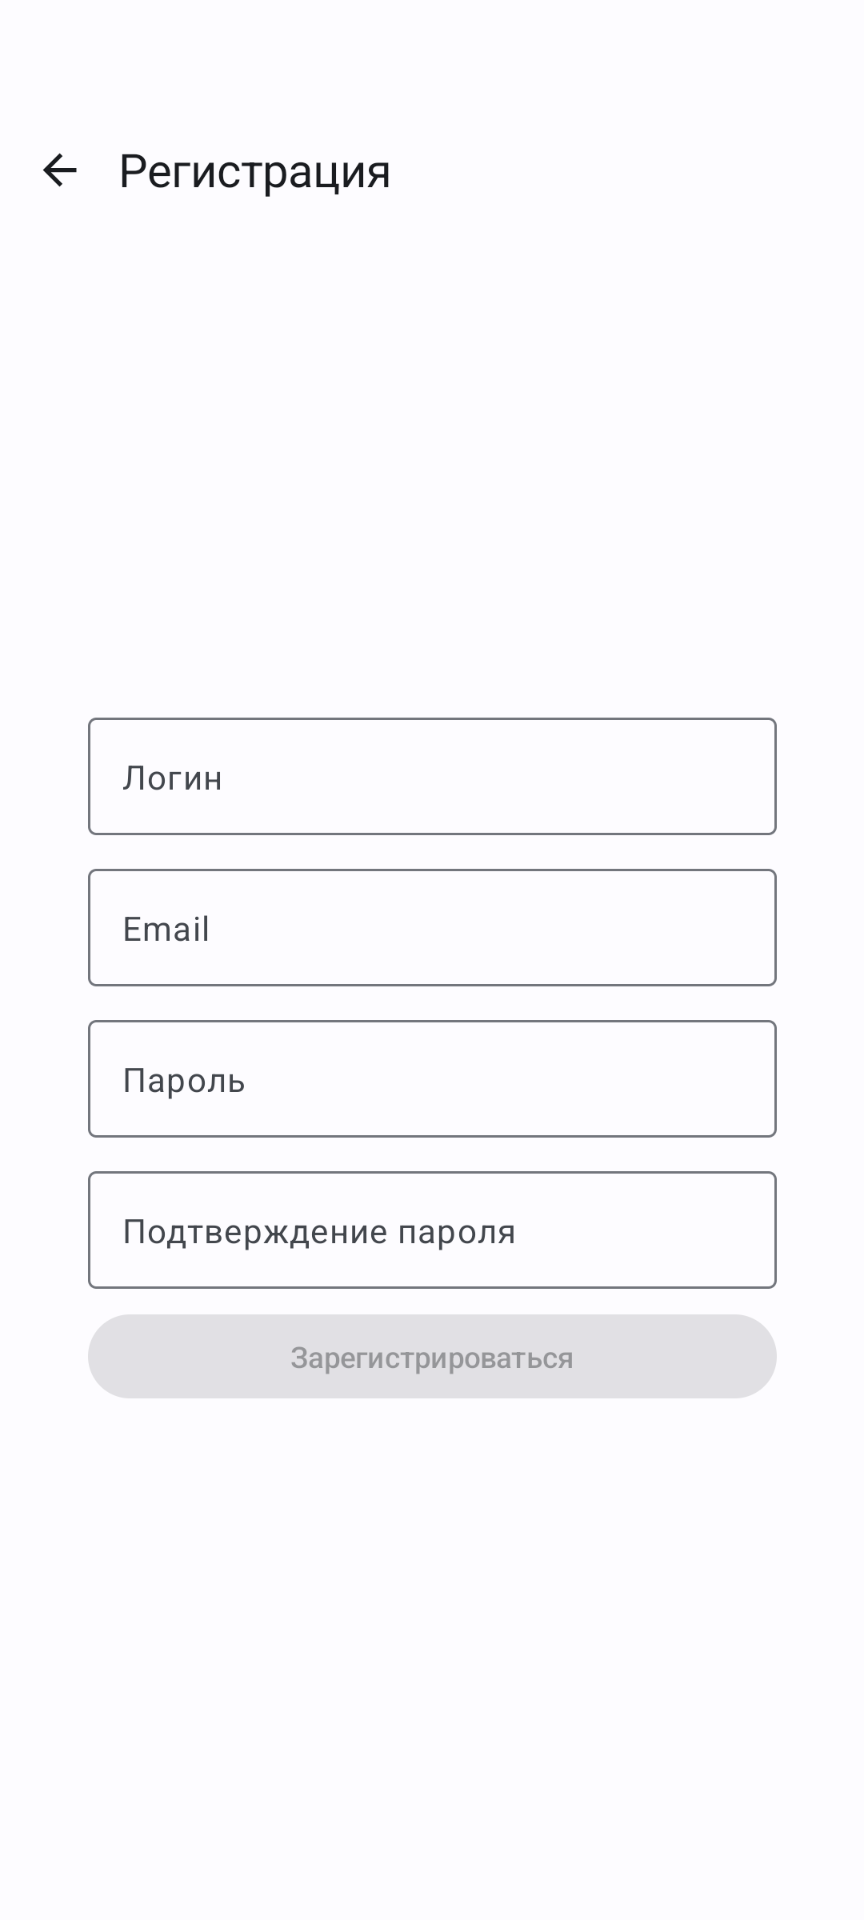
\includegraphics[width=5cm]{resources/6.png}
    \caption{Страница регистрации (RegistrationPage)}
\end{figure}

\begin{figure}[H]
    \centering
    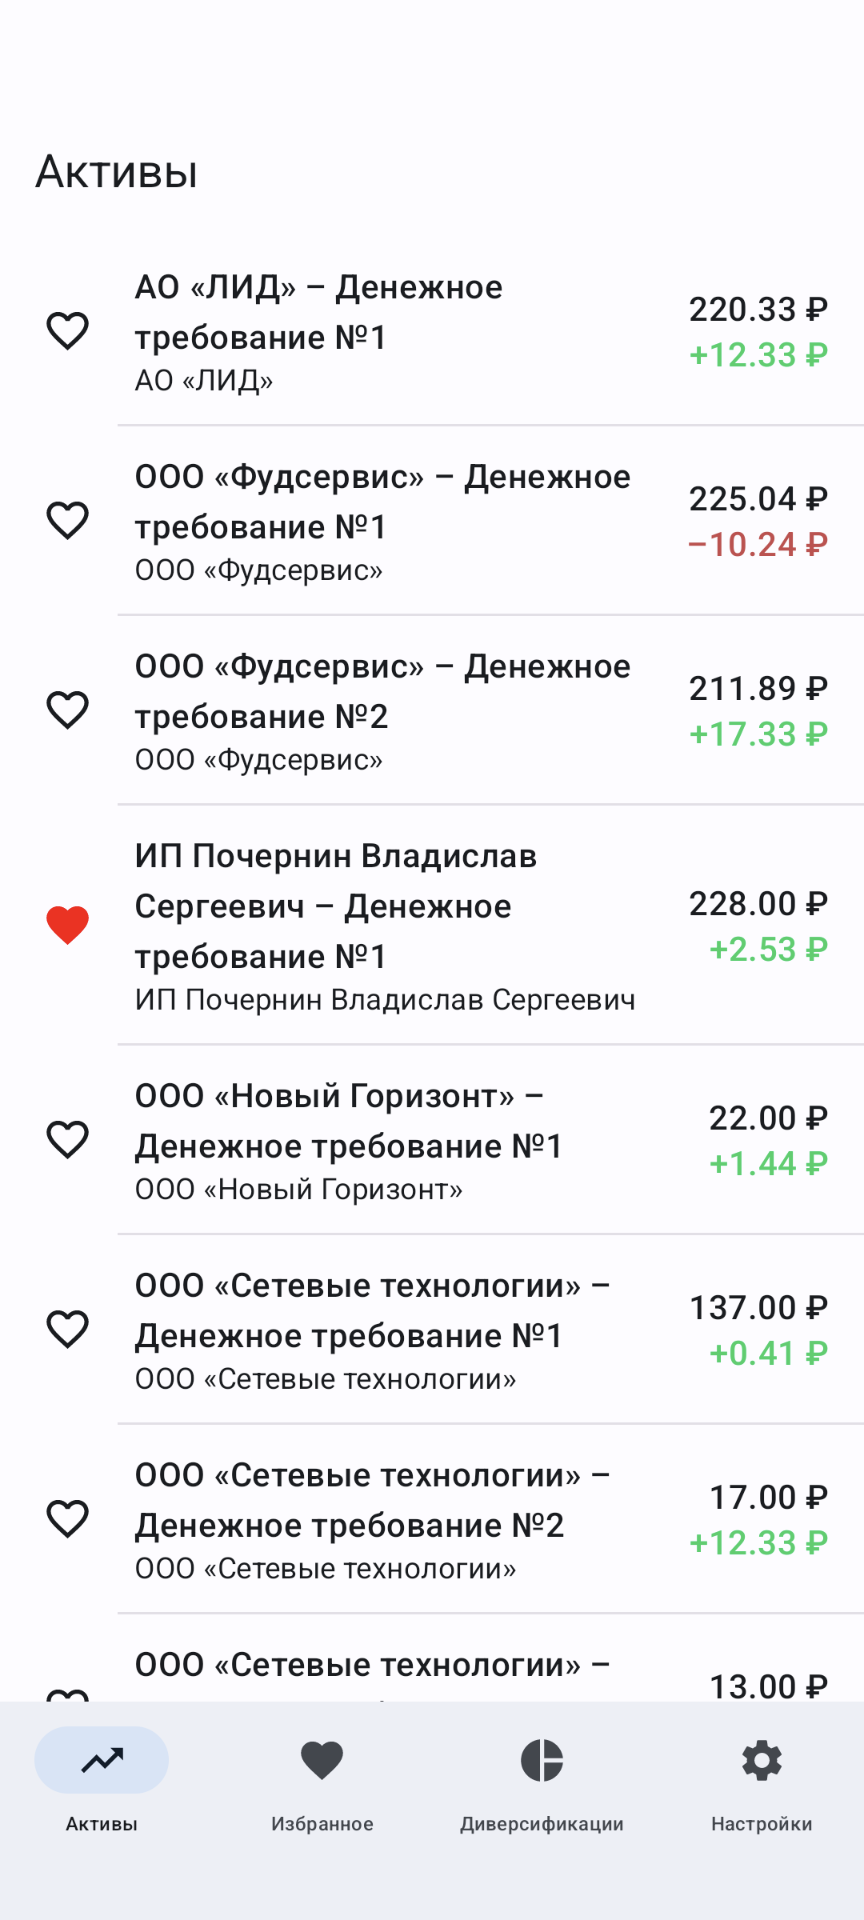
\includegraphics[width=5cm]{resources/7.png}
    \caption{Страница активов (AssetsPage)}
\end{figure}

\begin{figure}[H]
    \centering
    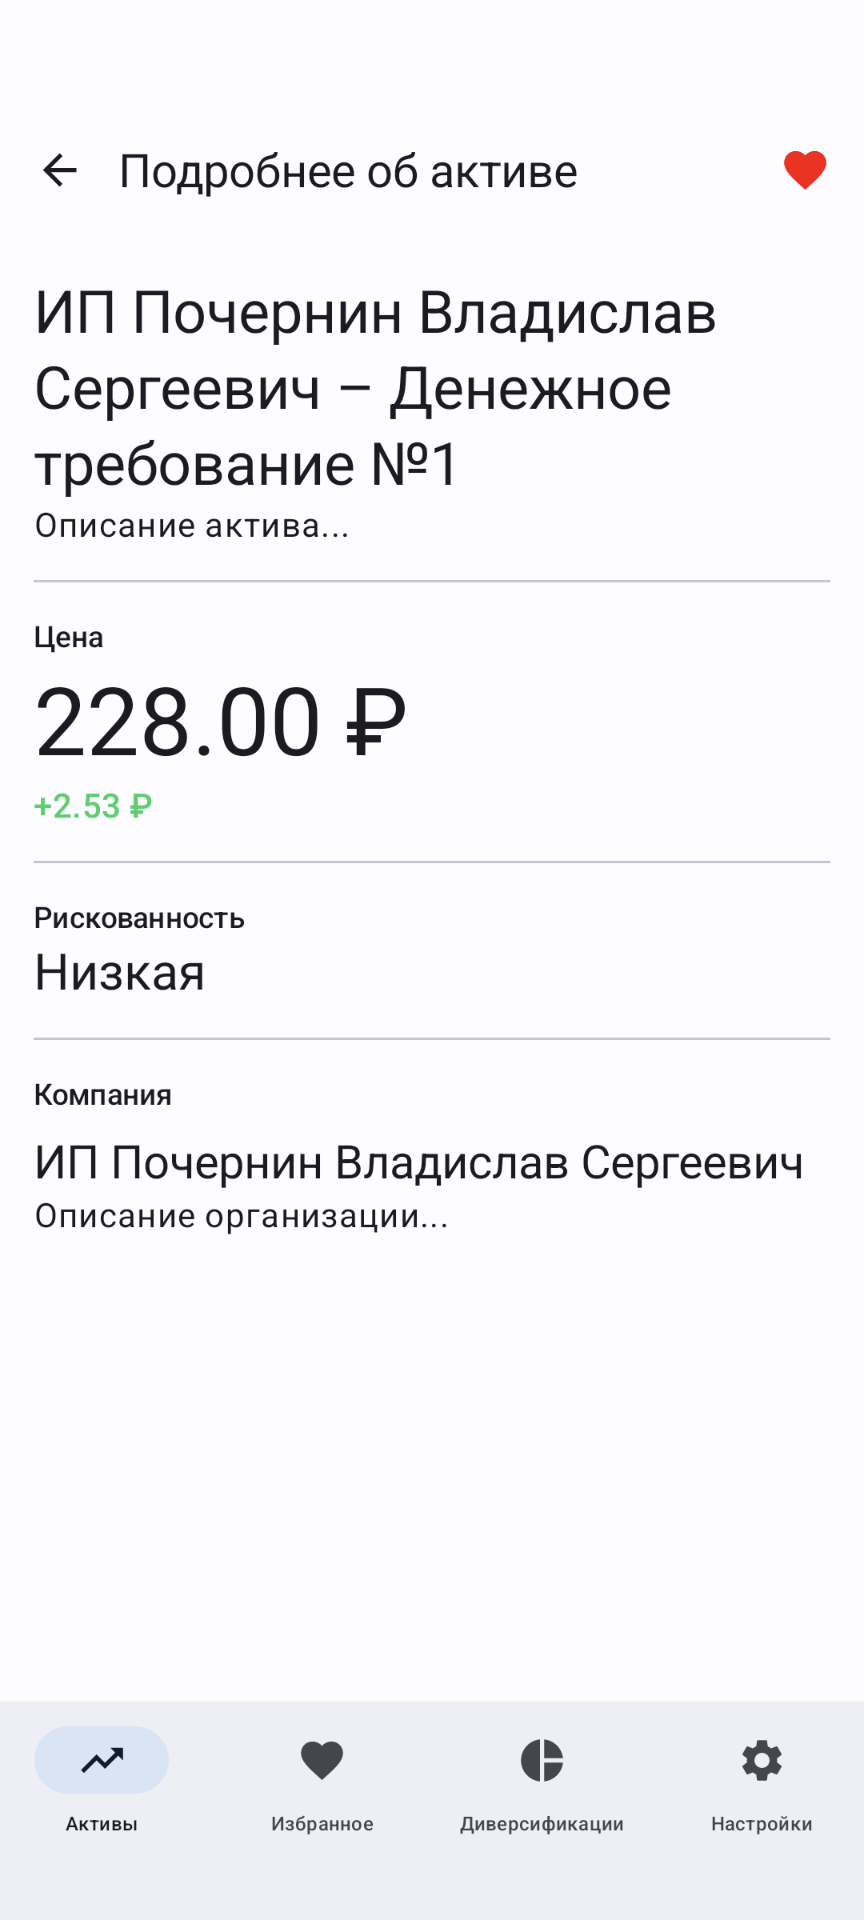
\includegraphics[width=5cm]{resources/8.png}
    \caption{Страница конкретного актива (AssetPage)}
\end{figure}

\begin{figure}[H]
    \centering
    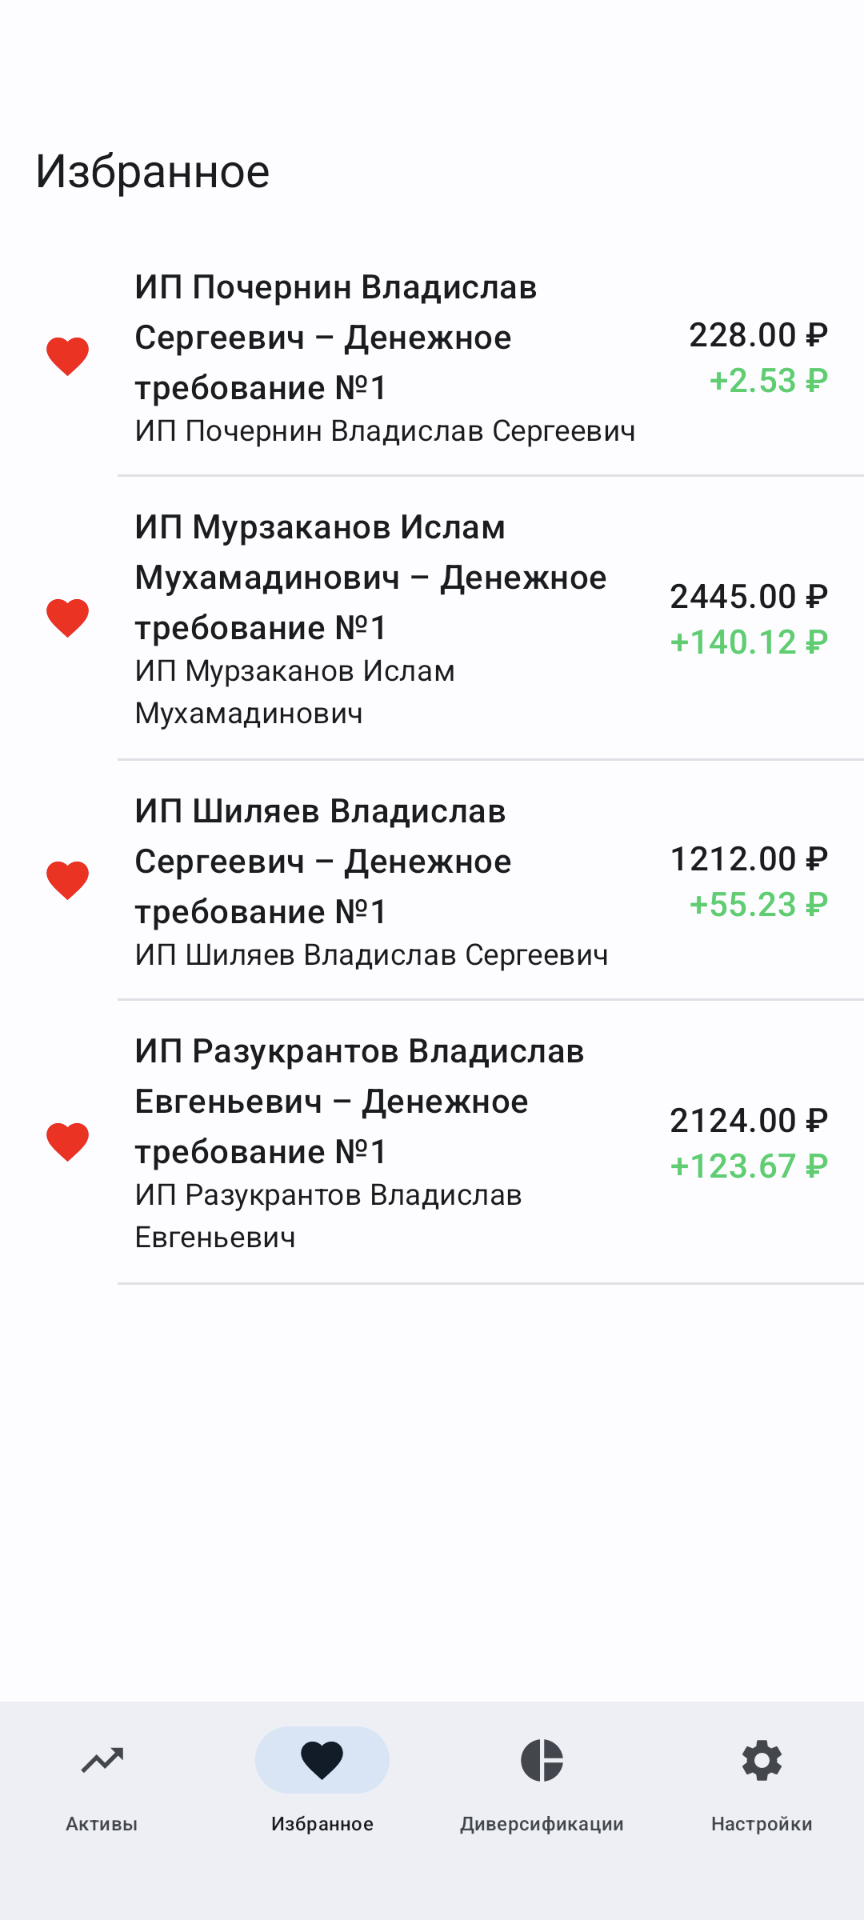
\includegraphics[width=5cm]{resources/9.png}
    \caption{Страница избранных активов (FavouritesPage)}
\end{figure}

\begin{figure}[H]
    \centering
    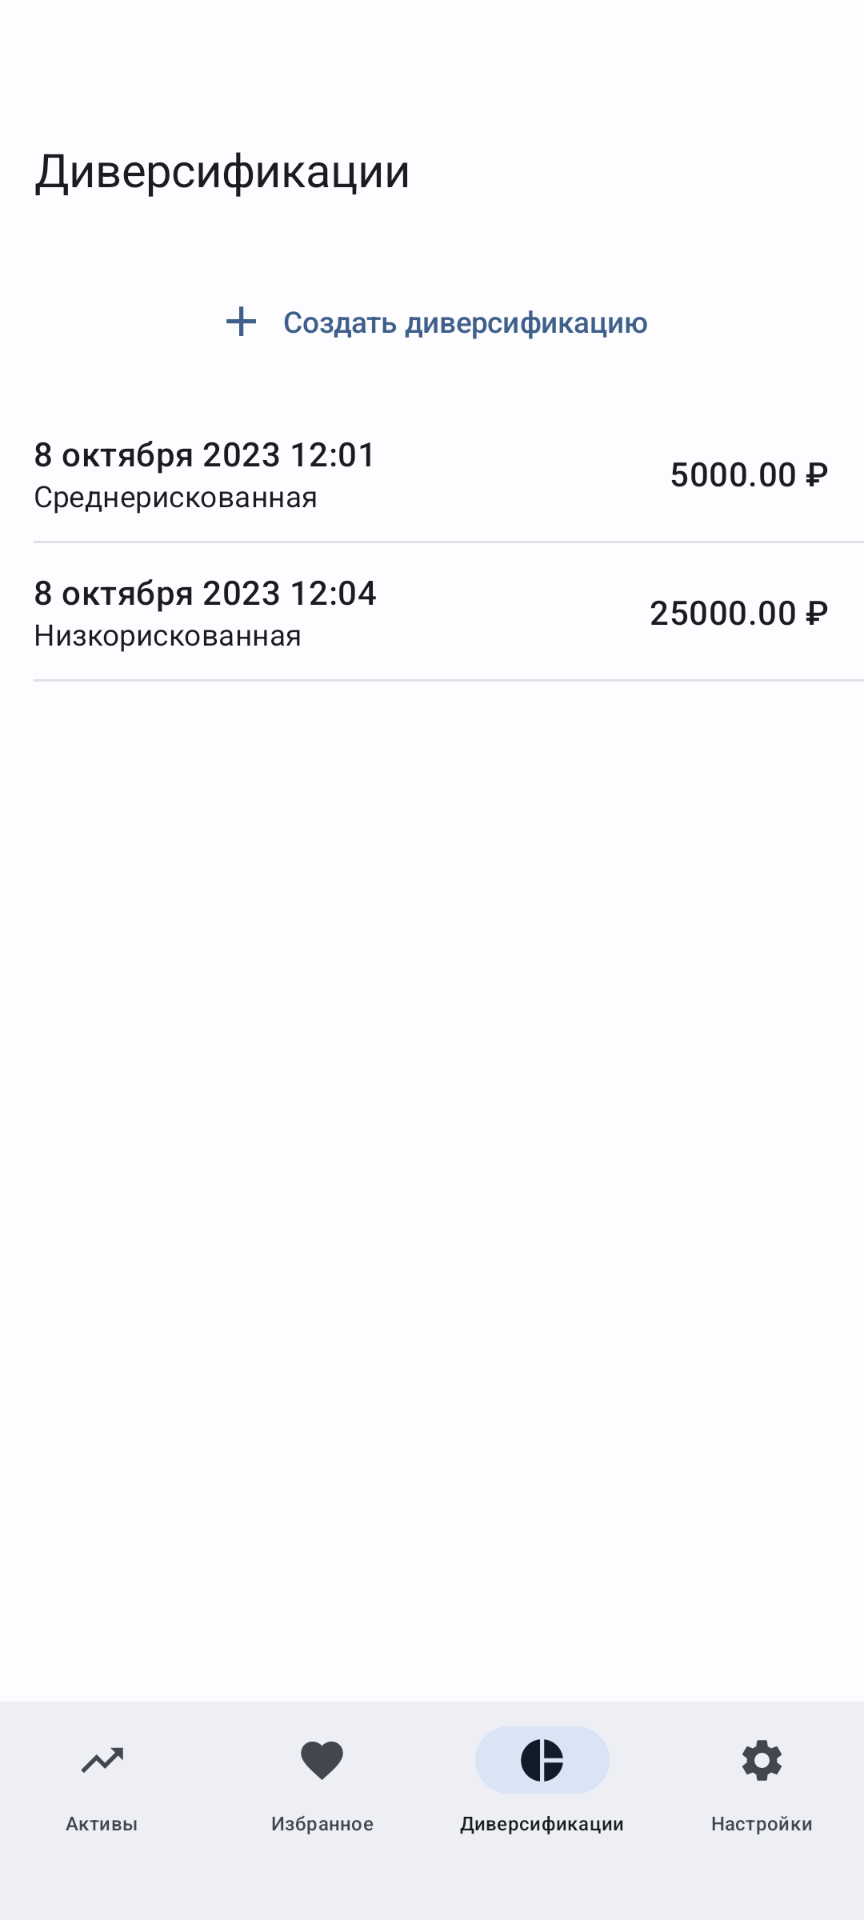
\includegraphics[width=5cm]{resources/10.png}
    \caption{Страница портфелей (PortfoliosPage)}
\end{figure}

\begin{figure}[H]
    \centering
    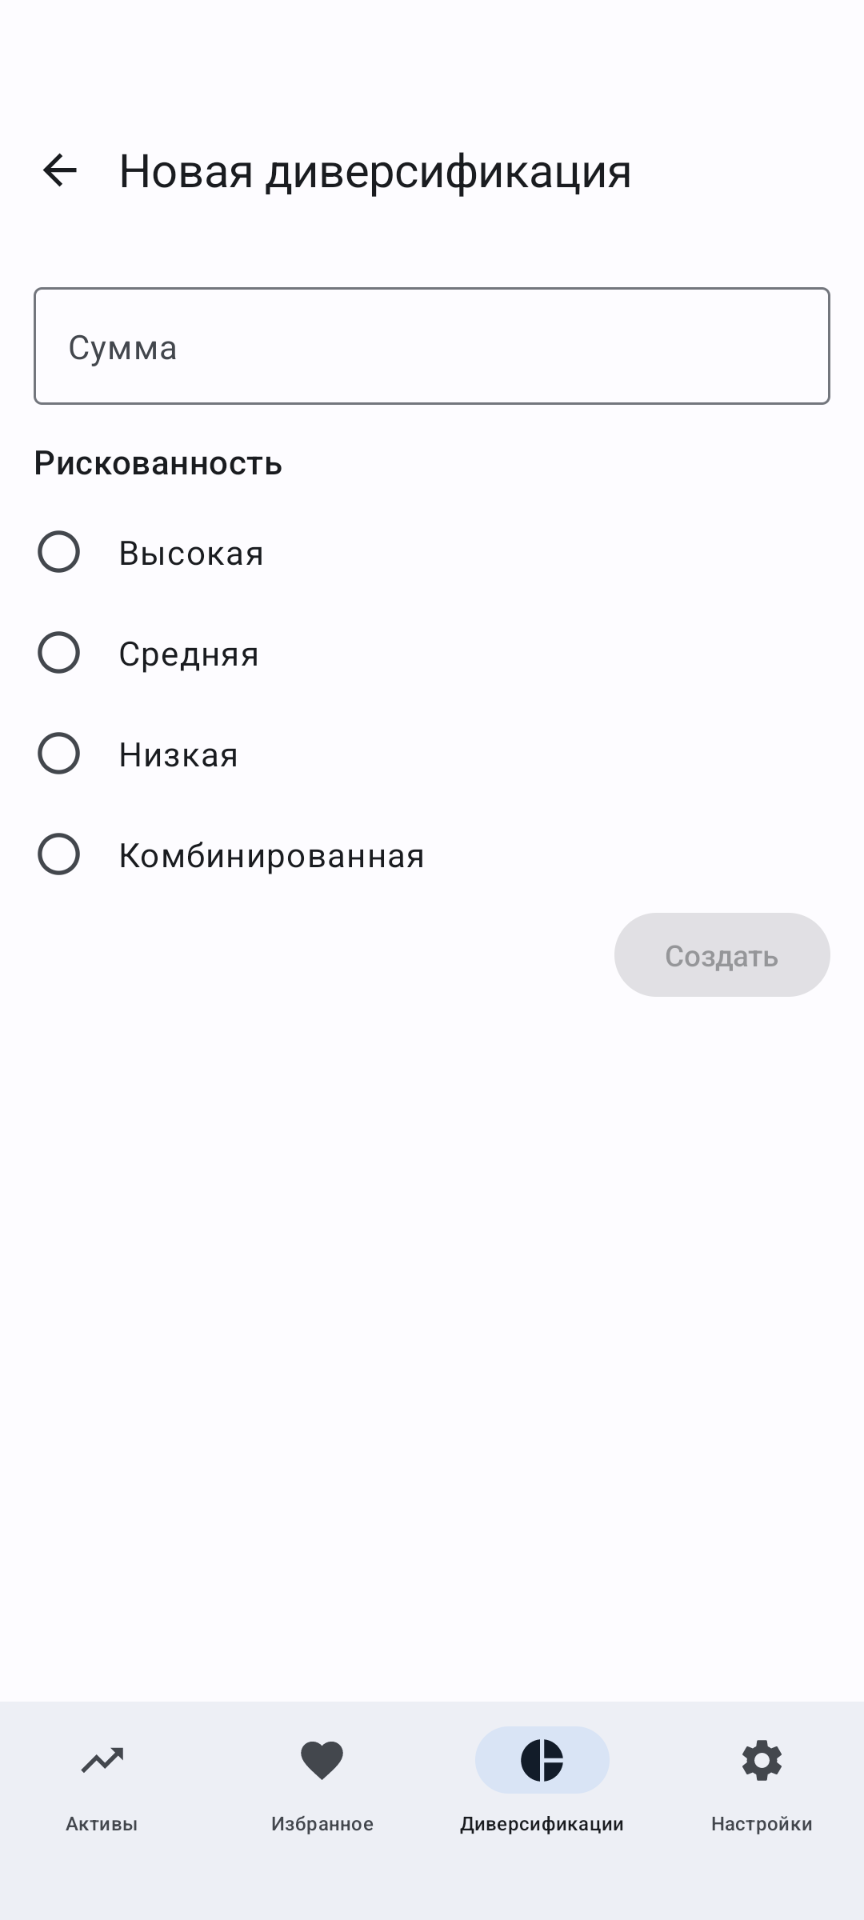
\includegraphics[width=5cm]{resources/11.png}
    \caption{Страница создания портфеля (PortfolioCreatePage)}
\end{figure}

\begin{figure}[H]
    \centering
    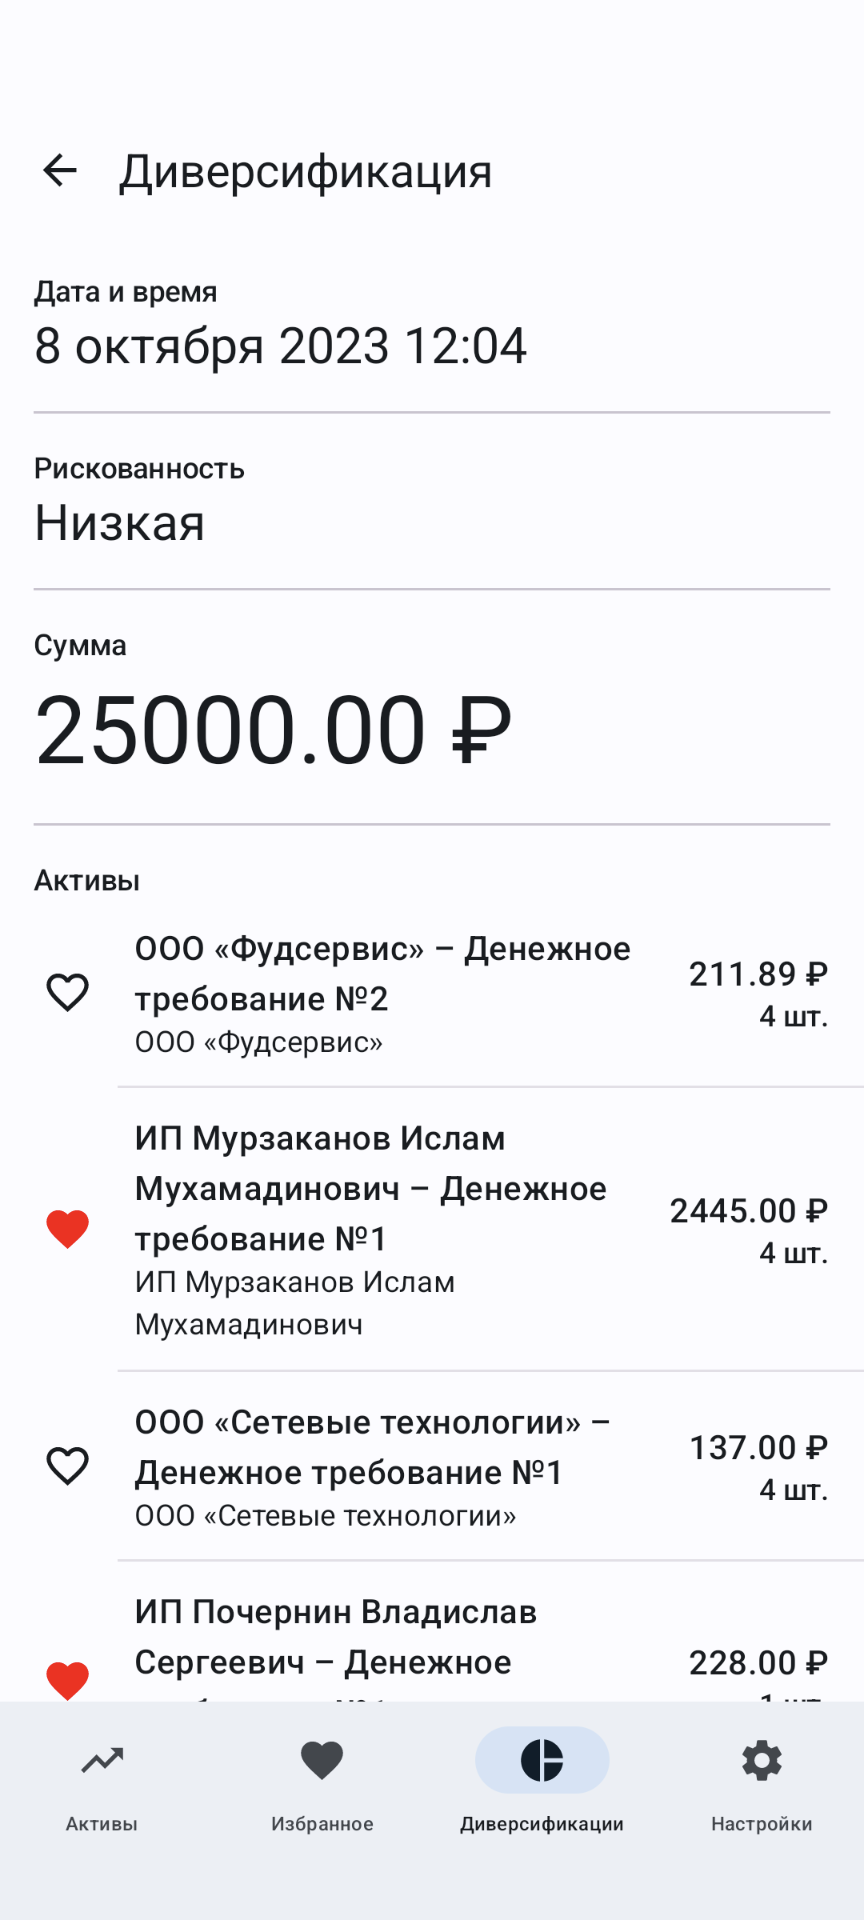
\includegraphics[width=5cm]{resources/12.png}
    \caption{Страница конкретного портфеля (PortfolioPage)}
\end{figure}

\begin{figure}[H]
    \centering
    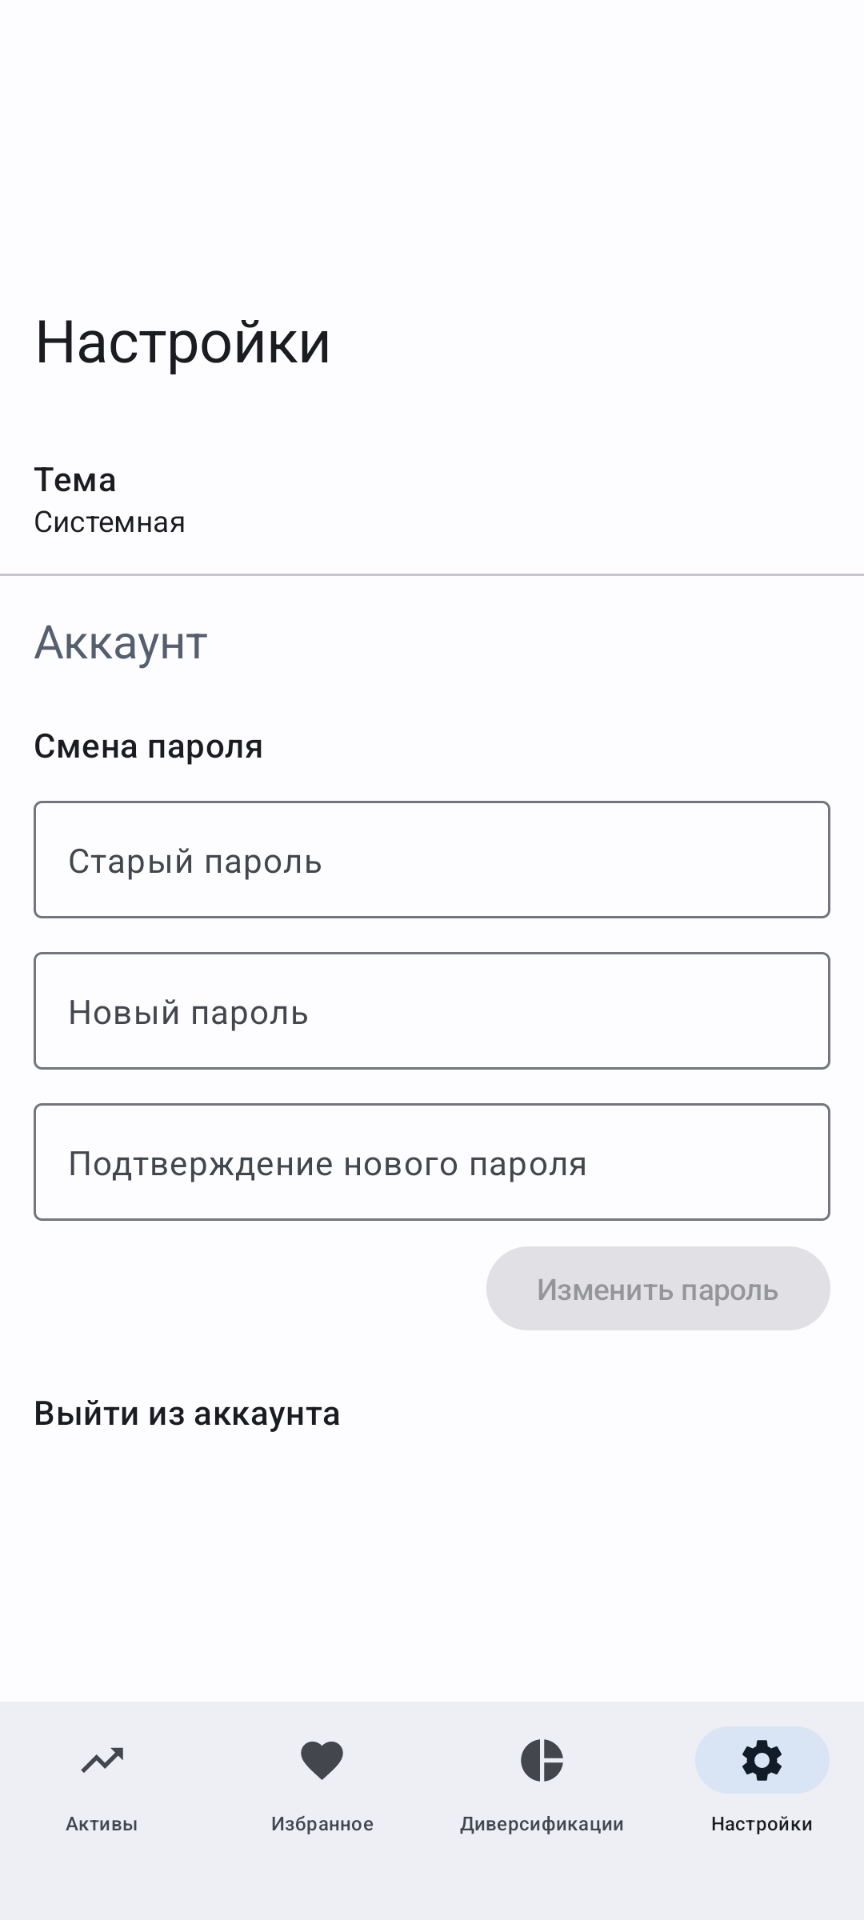
\includegraphics[width=5cm]{resources/13.png}
    \caption{Страница настроек (SettingsPage)}
\end{figure}

\end{document}